%
%   Prof. Dr. Julian Reichwald
%   auf Basis einer Vorlage von Prof. Dr. Jörg Baumgart
%   DHBW Mannheim
%


\documentclass[
	12pt,
	BCOR=5mm,
	DIV=12,
	headinclude=on,
	footinclude=off,
	parskip=half,
	bibliography=totoc,
	listof=entryprefix,
	toc=listof,
	pointlessnumbers,
	plainfootsepline]{scrreprt}

%	Konfigurationsdatei einziehen
%		LANGUAGE SETTINGS AND FONT ENCODING 
%
%\usepackage[ngerman]{babel} 	% German language
\usepackage[utf8]{inputenc}
%\usepackage[german=quotes]{csquotes} 	% correct quotes using \enquote{}
\usepackage[T1]{fontenc}


\usepackage[english]{babel}   % For english language
\usepackage{csquotes} 	% Richtiges Setzen der Anführungszeichen mit \enquote{}

% 		HYPERREF
%
\usepackage[
hidelinks=true % keine roten Markierungen bei Links
]{hyperref}

% Zwei eigene Befehle zum Setzen von Autor und Titel. Ausserdem werden die PDF-Informationen richtig gesetzt.
\newcommand{\TitelDerArbeit}[1]{\def\DerTitelDerArbeit{#1}\hypersetup{pdftitle={#1}}}
\newcommand{\AutorDerArbeit}[1]{\def\DerAutorDerArbeit{#1}\hypersetup{pdfauthor={#1}}}
\newcommand{\Firma}[1]{\def\DerNameDerFirma{#1}}
\newcommand{\Kurs}[1]{\def\DieKursbezeichnung{#1}}


% Correct superscripts 
\usepackage{fnpct}




%		CALCULATIONS
%
\usepackage{calc} % Used for extra space below footsepline
\usepackage{amsmath}
\usepackage{amssymb}
\usepackage{mathtools}


%		BIBLIOGRAPHY SETTINGS
%

% Uncomment the next three lines for author-year-style with footnotes (Chicago)
\usepackage[backend=biber, autocite=footnote, style=authoryear, dashed=false]{biblatex} 	%Use Author-Year-Cites with footnotes
\AdaptNoteOpt\footcite\multfootcite   %will add  separators if footcite is called multiple consecutive times 
\AdaptNoteOpt\autocite\multautocite % will add  separators if autocite is called multiple consecutive times

% Uncomment the next line for IEEE-style 
% \usepackage[backend=biber, autocite=inline, style=ieee]{biblatex} 	% Use IEEE-Style (e.g. [1])

% Uncomment the next line for alphabetic style 
% \usepackage[backend=biber, autocite=inline, style=alphabetic]{biblatex} 	% Use alphabetic style (e.g. [TGK12])

% Uncomment the next two lines vor Harvard-Style 
%\usepackage[backend=biber, style=apa]{biblatex} 	
%\DeclareLanguageMapping{german}{german-apa}


\DefineBibliographyStrings{ngerman}{  %Change u.a. to et al. (german only!)
	andothers = {{et\,al\adddot}},
}

%%% Uncomment the following lines to support hard URL breaks in bibliography 
%\apptocmd{\UrlBreaks}{\do\f\do\m}{}{}
%\setcounter{biburllcpenalty}{9000}% Kleinbuchstaben
%\setcounter{biburlucpenalty}{9000}% Großbuchstaben


\setlength{\bibparsep}{\parskip}		%add some space between biblatex entries in the bibliography
\addbibresource{bibliography.bib}	%Add file bibliography.bib as biblatex resource


%		FOOTNOTES 
%
% Count footnotes over chapters
\usepackage{chngcntr}
\counterwithout{footnote}{chapter}

%	ACRONYMS
%%%
%%% WICHTIG: Installieren Sie das neueste Acronyms-Paket!!!
%%%
\makeatletter
\usepackage[printonlyused]{acronym}
\@ifpackagelater{acronym}{2015/03/20}
{%
	\renewcommand*{\aclabelfont}[1]{\textbf{\textsf{\acsfont{#1}}}}
}%
{%
}%
\makeatother

%		LISTINGS
\usepackage{listings}	%Format Listings properly
\lstset{numbers=left,
	numberstyle=\tiny,
	captionpos=b,
	basicstyle=\ttfamily\small}


%		EXTRA PACKAGES
\usepackage{graphicx} % use various graphics formats
\usepackage[german]{varioref} 	% nicer references \vref
\usepackage{caption}	%better Captions
\usepackage{booktabs} %nicer Tabs
\usepackage{array}
\usepackage{tikz}
\usetikzlibrary{shapes,matrix,positioning, arrows.meta, fit}
\usepackage{pgfplots}
\usepackage{csvsimple}
\usepackage{xltabular}

%\newcolumntype{P}[1]{>{\raggedright\arraybackslash}p{#1}}


%		ALGORITHMS
\usepackage{algorithm}
\usepackage{algpseudocode}
\renewcommand{\listalgorithmname}{Algorithmenverzeichnis }
\floatname{algorithm}{Algorithmus}


%		FONT SELECTION: Entweder Latin Modern oder Times / Helvetica
\usepackage{lmodern} %Latin modern font
%\usepackage{mathptmx}  %Helvetica / Times New Roman fonts (2 lines)
%\usepackage[scaled=.92]{helvet} %Helvetica / Times New Roman fonts (2 lines)

%		PAGE HEADER / FOOTER
%	    Warning: There are some redefinitions throughout the master.tex-file!  DON'T CHANGE THESE REDEFINITIONS!
\RequirePackage[automark,headsepline,footsepline]{scrpage2}
\pagestyle{scrheadings}
\renewcommand*{\pnumfont}{\upshape\sffamily}
\renewcommand*{\headfont}{\upshape\sffamily}
\renewcommand*{\footfont}{\upshape\sffamily}
\renewcommand{\chaptermarkformat}{}
\RedeclareSectionCommand[beforeskip=0pt]{chapter}
\clearscrheadfoot

\ifoot[\rule{0pt}{\ht\strutbox+\dp\strutbox}DHBW Mannheim]{\rule{0pt}{\ht\strutbox+\dp\strutbox}DHBW Mannheim}
\ofoot[\rule{0pt}{\ht\strutbox+\dp\strutbox}\pagemark]{\rule{0pt}{\ht\strutbox+\dp\strutbox}\pagemark}

\ohead{\headmark}

\begin{document}

\TitelDerArbeit{Neural Networks for Tool Image Classification}
\AutorDerArbeit{Fabian Wolf}
\Firma{Movilizer GmbH}
\Kurs{WWI17SEC}

\begin{titlepage}
\begin{minipage}{\textwidth}
		\vspace{-2cm}
		\noindent 
\includegraphics[scale=0.71]{img/firmenlogo.pdf} \hfill   
\includegraphics{img/dhbwlogo.pdf}
\end{minipage}
\vspace{1em}
\sffamily
\begin{center}
	\textsf{\large{}Duale Hochschule Baden-W\"urttemberg\\[1.5mm] Mannheim}\\[2em]
	\textsf{\textbf{\Large{}Bachelor Thesis}}\\[3mm]
	\textsf{\textbf{\DerTitelDerArbeit}} \\[1.5cm]
	\textsf{\textbf{\Large{}Course of Study: Business Informatics}\\[3mm] \textsf{Field of Study: Software Engineering}}
	
%	\vspace{3em}
%	\textsf{\Large{Sperrvermerk}}
\vfill

\begin{minipage}{\textwidth}

\begin{tabbing}
	Spacing Spacing Spacing: \hspace{0.85cm}\=\kill
	Author: \> \DerAutorDerArbeit \\[1.5mm]
	Matriculation Number: \> 7345461 \\[1.5mm]
	Company: \> \DerNameDerFirma  \\[1.5mm]
	Department: \> Research and Development \\[1.5mm]
	Course of Study: \> \DieKursbezeichnung \\[1.5mm]
	Head of Course of Study: \> Prof. Dr.-Ing. habil. Dennis Pfisterer  \\[1.5mm]
	Scientific Supervisor: \> M.Sc. Boas Bamberger  \\
	\> bamberger@uni-mannheim.de \\
	\> +49 621 181 1562 \\[1.5mm]
	Business Supervisor: \> Oliver Erlenkaemper \\
	\> oliver.erlenkaemper@honeywell.com \\
	\> +49 621 150 207 36 \\[1.5mm]
	Processing Period: \> 02 March 2020--11 May 2020 
\end{tabbing}
\end{minipage}

\end{center}

\end{titlepage}

\pagenumbering{roman}
\normalfont

%--------------------------------
% PRE TEXTS
%--------------------------------
%	Kurzfassung
\chapter*{Abstract}
\begingroup
\begin{table}[h!]
\setlength\tabcolsep{0pt}
\begin{tabular}{p{3.7cm}p{11.7cm}}
Title & \DerTitelDerArbeit \\
Author: & \DerAutorDerArbeit \\
Course of Study: & \DieKursbezeichnung \\
Company: & \DerNameDerFirma\\
\end{tabular}
\end{table}
\endgroup


% Problemstellung
The career guidance provider Aivy receives recruitment advertisements from several companies, so those of interest for Aivy's customers can be forwarded to them. In order to exclusively forward the recruitment advertisements of interest, they need to be classified first. Manual classification creates expensive and recurrent costs, while the implementation of a neural classification model substituting human labor is a one-time investment. On that account, a neural model holds the potential of significant cost reduction.
% Forschungsziel
This paper seeks to propose a neural model for the recruitment advertisement classification task.
% Methode
Therefore, state of the art models for neural text classification are discussed in regard to the requirements of the recruitment advertisement classification task. The state of the art on neural text classification is captured by the literature review conducted by this paper. The requirements are derived from the recruitment advertisement classification task.
% Ergebnis
In general, any state of the art model for text classification satisfies the requirements. Accordingly, no model can be excluded based on the requirements. However, XLNet is the on average best performing model on several text classification leaderboards.\footnote{\url{https://gluebenchmark.com/leaderboard/}}\footnote{\url{https://nlpprogress.com/english/text_classification.html}}\footnote{\url{https://paperswithcode.com/sota}}. Furthermore, XLNet is available under Apache License 2.0. This license allows for commercial use free of charge.
% Resultierende Empfehlung
For this reason, this paper proposes the pre-trained XLNet fine-tuned on the recruitment advertisement classification task for this task.

%	Inhaltsverzeichnis
\tableofcontents

%	Abbildungsverzeichnis
\listoffigures

%	Tabellenverzeichnis
\listoftables

% Algorithmenverzeichnis
\renewcommand{\listalgorithmname}{List of Algorithms}
\listofalgorithms

% 	Abkürzungsverzeichnis (siehe Datei acronyms.tex!)
%\addcontentsline{toc}{chapter}{Acronyms}
\clearpage
\chapter*{Acronyms}	
\addcontentsline{toc}{chapter}{Acronyms}


\begin{acronym}[RDBMS]
	\acro{API}{Application Programming Interface}
	\acro{AWS}{Amazon Web Service}
	\acro{CNN}{Convolutional Neural Network}
	\acro{GRU}{Gated Recurrent Unit}
	\acro{LSTM}{Long Short-Term Memory}
	\acro{MLP}{Multi Layer Perzeptron}
	\acro{NLP}{Natural Language Processing}
	\acro{ReLU}{Rectified Linear Unit}
	\acro{RNN}{Recurrent Neural Network}
\end{acronym}

\ohead{Acronyms} % Neue Header-Definition


%--------------------------------
% MAIN TEXTS
%--------------------------------
\clearpage
\ihead{\chaptername~\thechapter}
\ohead{\headmark}
\pagenumbering{arabic}
\chapter{Introduction}

\section{Motivation}
\label{sec:motivation}
% AR
\blockquote[\cite{Detzel.2018}]{It might take two hours for an experienced field technician to fix a broken MRI. But a pair of smart glasses that displays step-by-step instructions in the tech’s field of vision could help shave as much as 50\% from the time it takes to diagnose the problems and make needed repairs.} According to Boston Consulting Group, Accenture, Mc Kinsey, and others, augmented reality solutions for field workers are an emerging market. \autocites{EY.2019a}{EY.2019b}{Detzel.2018}{Shook.2019}{Guy.2019} The augmented reality market is estimated to reach 83.5 billion USD by 2021. \autocite{Statista.2019} Movilizer GmbH approaches this trend with its connected solutions. \autocites{Honeywell.2018a}{Honeywell.2018b}
An augmented reality solution for field workers requires software perceiving the environment of field workers. A sub-task of that perception is to distinguish tools of different classes. For example, a software displaying step-by-step instructions in the field of vision of a field worker needs to distinguish a screwdriver from a wrench when telling the field worker to tighten the screw with the wrench lying on the ground next to him instead of the screwdriver in his hand.
% Neural Networks
Distinguishing between tools of different classes is called tool image classification. Image classification in general is mostly solved by neural networks. \autocites{ElAmir.2020}{LeCun.2015}{Singh.2020}{Michelucci.2019}{Gad.2018}{Kapur.2017} 
% Research Questions
This paper determines the best-performing neural network for tool image classification. Furthermore, this paper introduces a novel tool image classification dataset called \ac{TIC Dataset}.



\section{Problem Statement}
\label{sec:problem}
Tool image classification is the problem of assigning the correct class to an image of a tool, see Section \ref{sec:ml}. An image of a tool is a close-up image of exactly one tool from an arbitrary angle with an arbitrary background. To classify an image, a neural network receives an image and returns the class probabilities. The class with the highest probability is the prediction of the neural network for that image.
A $w$-by-$h$-pixel image is formatted as three-dimensional array. The array contains one subarray for each pixel. The $X$ and $Y$ coordinates of a pixel in an image correspond to the indices of the subarray containing the $d$ color values of that pixel. Consequently, the three-dimensional array is of shape $w \times h \times d$. \autocites{LeCun.2015b}{LeCun.1998} For example, a three-color, $224$-by-$224$-pixel image is formatted as an array of shape $224 \times 224 \times 3$. The class probabilities are formatted as a one-dimensional array. Each index of that array corresponds to one class. The element at a given index is the class probability of the corresponding class. \autocite{ElAmir.2020} For example, a class array for the classes screwdriver and wrench is of shape $2$. Index~$0$ corresponds to screwdriver and index $1$ corresponds to wrench.
\par
To classify correctly, neural networks need to be trained first. \autocite{ElAmir.2020} This paper trains and evaluates neural networks on the \ac{TIC Dataset}.  The \ac{TIC Dataset} is constructed by this paper and comprises $20{,}400$ tool images of six classes. The classes are listed below.
\begin{itemize}
	\item drill
	\item hammer
	\item pliers
	\item saw
	\item screwdriver
	\item wrench
\end{itemize}
Each class comprises $3{,}400$ tool images. A tool image is a close-up image of exactly one tool. 
For a class, tool images display different tools of the same class from arbitrary angles and with arbitrary backgrounds. 



\section{Scope}
\label{sec:scope}
Summarizing, the scope of this paper is to determine the best-performing neural network for tool image classification. On that account, this paper focuses on neural networks for image classification. 
Time and resources of this paper are limited. For this reason, the neural networks are trained exclusively supervised without auxiliaries.
% Exclusion
On that account, the following approaches and techniques are excluded. Metalearning is excluded. Non-neural networks are excluded. Other computer vision tasks are excluded. Unsupervised learning and semi-supervised learning are excluded. Auxiliaries used to improve the learning of neural networks are excluded. 
% Metalearning
Metalearning is the process of learning to learn, for example, learning hyperparameters of a neural network such as the architecture of the network using an evolutionary algorithm. \autocite{Schaul.2010}
% Non-Neural Networks
This paper regards several approaches as non-neural networks. These approaches are neural networks augmented with other machine learning algorithms, other machine learning algorithms in general or other image classification methods.
% Other Computer vision tasks
Computer vision tasks other than image classification are excluded because they are less related to the problem investigated in this paper than image classification.
% Un/Semisupervised
Semi-supervised or unsupervised learning is learning without knowing all or any desired output. \autocite{ElAmir.2020}
% Auxiliaries
This paper regards transfer learning, adversarial training, data augmentation, input normalization, weight decay, and multi-task learning as learning auxiliaries. 
Transfer learning aims to help learning a specific task by learning another task. For example, learning classification of geometric shapes in images might help learning tool image classification. 
\autocite{Pan.2010}
Adversarial training is training neural networks on adversarial examples. Adversarial examples are imperceptibly, non-randomly perturbed images. The perturbation arbitrarily changes the prediction of the neural network. \autocite{Szegedy.2014}
Data augmentation is the creation of additional training data from existing training data, for example, creating additional training images by rotating them by a random amount. 
\autocite{ElAmir.2020}
Input normalization improves training by re-scaling all input data into the same scale. 
\autocite{ElAmir.2020}
Weight decay improves training by penalizing large weights. 
\autocite{ElAmir.2020}
Mulit-task learning allows neural networks to learn multiple objectives. Hence, one loss function per objective is optimized during training.\autocite{Caruana.1997} For example, \cite{Sabour.2017} made their neural network learn image classification and reconstruction of the original input.

\section{Approach}
This paper seeks to determine the best-performing neural network for tool image classification. The best-performing neural network for tool image classification is determined in the course of an experiment. The experiment trains and evaluates state-of-the-art neural networks for image classification on the \ac{TIC Dataset}. The evaluation is based on a metric. The metric is determined based on the metrics used by image classification leaderboards. The state-of-the-art neural networks are determined in the course of a literature review conducted by this paper. The \ac{TIC Dataset} is constructed in the course of this paper.

\section{Structure}
The following chapters of this paper are structured as follows. 
\begin{itemize}
	\item Chapter \ref{chp:funda} defines and illustrates terms required to understand this paper.
	\item Chapter \ref{chp:metho} defines the methodology followed to determine the best-performing neural network for tool image classification.
	\item Chapter \ref{chp:sota} reports the results of the literature review on the state of the art of image classification conducted by this paper.
	\item Chapter \ref{chp:result} reports the results of the experiment conducted by this paper.
	\item Chapter \ref{chp:discussion} discusses the results of the experiment conducted by this paper. Furthermore, the work of this paper is placed in the state of the art of image classification, and the limitations of this work are reflected. Finally, future work and practical implications are proposed.
	\item Chapter \ref{chp:conclusion} summarizes the contributions of this paper.
\end{itemize}
\chapter{Fundamentals}
\label{ch:fundamentals}
	Understanding this paper requires knowledge about certain terms. These terms are defined and illustrated in this chapter.

	\section{Text Classification}
	\label{sec:classification}
		Text classification is a special topic within the more general field of text mining which tries to extract useful information from unstructured texts.\autocite{Baharudin.2010} Text classification does this by labeling a text with its corresponding class labels. A text can correspond to only one class (single-label) or more classes (multi-label). Assigning only one label out of several classes is called multi-class classification while assigning several labels is called multi-label classification.
		\par
		It is common to represent the class distribution of a text with a one-hot array for multi-class classification or a multi-hot array for multi-label classification. Each scalar of the vector represents the probability of a given class. For example, imagine classifying recruitment advertisements for baker, barber and butcher. In this example the class distribution vector has three scalars the first one corresponding to baker, the second one to barber and the third one to butcher. In consequence, a golden vector for a bakers recruitment advertisement looks like \eqref{eq:1hot}.
		\begin{equation}
			\label{eq:1hot}
			\begin{pmatrix}
				1\\
				0\\
				0\\
			\end{pmatrix}
		\end{equation}
		For neural multi-class classification this is achieved using the softmax activation function. The softmax function represents a probability distribution over all classes. Therefore, the golden vector has the probability $1$ for the recruitment advertisements class and $0$ for all other classes. As the predicted vector is most likely not equal to the golden vector, the class with the highest scalar value is taken as the predicted class.\autocite{Krause.2017}
		For multi-label classification this does not work, as the golden vector can contain several probabilities of $1$. Because of this the sigmoid or logistics activation function is used. The sigmoid activation function \enquote{squashes} all values into the range $[0;1]$. \autocite{Krause.2017} Here again, the predicted vector is most likely not equal to the golden vector. That is why a threshold is used to decide whether a classes is taken as predicted or not. All classes with a corresponding scalar value above a certain threshold are taken as predicted. \autocite{LeCun.2015}

	\section{Neuron}
		\label{sec:neuron}
		A neuron is the basic unit of a neural network. A neuron consists of  $n$ weighted connections  $w_i, i \in [1;n]$, a sum function $\sum$ and an activation function $\varphi$\autocite{Jain.1996}, see Figure \ref{img:neuron}. Common activation functions are sigmoid, tanh and \ac{ReLU}. In recent years \ac{ReLU} is commonly used.\autocite{LeCun.2015} Chaining these operations produces the output $y$ of a neuron. Given an input $\vec{x}$ this operator chain results in Equation \eqref{eq:neuron:y}.\autocite{Jain.1996}
		\begin{equation}
			\label{eq:neuron:y}
			\begin{array}{lcl}
			y & = & \varphi(\sum_{i=1}^{n} x_i \cdot w_i)\\
			& = & \varphi(\vec{w}^{\mathrm {T}} \cdot \vec{x}) | \vec{w}^{\mathrm {T}}=(w_1, w_2 \dots w_n)
			\end{array}
			\end{equation}
		\begin{figure}[H]
			\centering
			\begin{tikzpicture}
			\node (x0) at (0,3) {$x_0$};
			\node (x1) at (0,2) {$x_1$};
			\node (..) at (0,1) {$\vdots$};
			\node (xn) at (0,0) {$x_n$};
			\node[draw, circle, minimum size=1cm] (sum) at (2,1.5) {$\sum$};
			\node[draw, circle, minimum size=1cm] (phi) at (4,1.5) {$\varphi$};
			\node (y) at (6,1.5) {$y$};
			\draw[->] (x0) -- (sum) node[sloped,pos=.3,above] {$w_0$};
			\draw[->] (x1) -- (sum) node[sloped,pos=.3,above] {$w_1$};
			\draw[->] (xn) -- (sum) node[sloped,pos=.3,above] {$w_n$};
			\draw[->] (sum) -- (phi);
			\draw[->] (phi) -- (y);
			\node[draw,	ellipse, minimum height=2cm,minimum width=3cm, label=Neuron] (neuron) at (3,1.5) {};
			\end{tikzpicture}
			\caption{Neuron (own figure)} \label{img:neuron}
		\end{figure}

	\section{\ac{MLP}}
	\label{sec:mlp}
		A \ac{MLP} or multilayer feed forward network is a basic neural network structure. A \ac{MLP} consists of interconnected neurons. The neurons are arranged in $m$ layers $l \in [0,m]$. A layer can contain any number $n$ of neurons. Each neuron of layer $l$ is connected to each neuron in layer $l-1$, see Figure \ref{img:nnexample}. \autocite{Svozil.1997} The connections between two layers can be described in a matrix. Given the neurons $n_{kl}$ in row $k, k \in [0,n]$ of layer $l$, the weight $w_{ij}$ describes the connection between the neuron $n_{jl-1}$ in row $j$ of the previous layer $l-1$ and the neurons $n_{il}$ in row $i$ of the layer $l$. In consequence, each layer possesses an own weight matrix $W_l$. In this matrix the weights describing all incoming connections of a neuron $n_{kl}$ are arranged in row $k$. This row corresponds to the transposed weight vector of a neuron $\vec{w}^{\mathrm {T}}$, as described in Equation \eqref{eq:neuron:y}. Resulting therefrom, applying an element wise activation function to the product of the weight matrix $W_l$ and the input vector $\vec{x_l}$ of a layer results in the output vector of that layer $\vec{y_l}$. This operation chain is described by Equation \ref{eq:nn:y}. Consequently, this equation can be seen as applying a linear vector space transformation followed by a non linear vector space transformation of the layers input.
		\begin{equation}
			\label{eq:nn:y}
			\vec{y_l} = \varphi(W_l \cdot \vec{x_l})
		\end{equation}
		\begin{figure}[H]
			\centering
			\begin{tikzpicture}
				% input
				\node (x0) at (0,3) {$x_0$};
				\node (x1) at (0,1.5) {$x_1$};
				\node (x2) at (0,0) {$x_2$};
				% input layer
				\node[align=center, text width=20em] (ins) at (3.5,4.5) {input layer};
				\node[draw, circle, minimum size=1cm] (n00) at (3.5,3) {$n_{00}$};
				\node[draw, circle, minimum size=1cm] (n10) at (3.5,1.5) {$n_{10}$};
				\node[draw, circle, minimum size=1cm] (n20) at (3.5,0) {$n_{20}$};
				% hidden layer
				\node[align=center, text width=20em] (hs) at (7,4.5) {hidden layer};
				\node[draw, circle, minimum size=1cm] (n01) at (7,2.25) {$n_{01}$};
				\node[draw, circle, minimum size=1cm] (n11) at (7,0.75) {$n_{11}$};
				% output layer
				\node[align=center, text width=20em] (hs) at (10.5,4.5) {outputlayer};
				\node[draw, circle, minimum size=1cm] (n02) at (10.5,1.5) {$n_{02}$};
				% output
				\node (y) at (14,1.5) {$y_0$};
				% input -> input layer
				\draw[->] (x0) -- (n00) node[sloped,pos=.50,above] {$w_{00}$};
				\draw[->] (x0) -- (n10) node[sloped,pos=.40,above] {$w_{10}$};
				\draw[->] (x0) -- (n20) node[sloped,pos=.70,above] {$w_{20}$};
				\draw[->] (x1) -- (n00) node[sloped,pos=.25,above] {$w_{01}$};
				\draw[->] (x1) -- (n10) node[sloped,pos=.40,above] {$w_{11}$};
				\draw[->] (x1) -- (n20) node[sloped,pos=.25,above] {$w_{21}$};
				\draw[->] (x2) -- (n00) node[sloped,pos=.70,above] {$w_{02}$};
				\draw[->] (x2) -- (n10) node[sloped,pos=.40,above] {$w_{12}$};
				\draw[->] (x2) -- (n20) node[sloped,pos=.50,above] {$w_{22}$};
				% input layer -> hidden layer
				\draw[->] (n00) -- (n01) node[sloped,pos=.5,above] {$w_{00}$};
				\draw[->] (n00) -- (n11) node[sloped,pos=.6,above] {$w_{10}$};
				\draw[->] (n10) -- (n01) node[sloped,pos=.2,above] {$w_{01}$};
				\draw[->] (n10) -- (n11) node[sloped,pos=.2,above] {$w_{11}$};
				\draw[->] (n20) -- (n01) node[sloped,pos=.6,above] {$w_{02}$};
				\draw[->] (n20) -- (n11) node[sloped,pos=.5,above] {$w_{12}$};
				% hidden layer -> output layer
				\draw[->] (n01) -- (n02) node[sloped,pos=.5,above] {$w_{00}$};
				\draw[->] (n11) -- (n02) node[sloped,pos=.5,above] {$w_{01}$};
				% output layer -> output
				\draw[->] (n02) -- (y);
			\end{tikzpicture}
			\caption{\ac{MLP} Illustration (own figure)} \label{img:nnexample}
		\end{figure}
		\par
		Figure \ref{fig:nn_matrix} illustrate the transfer of the connections between two layers to their matrix representation. In this illustration all incoming connections of a neuron are highlighted in the same color. These connections are described by the transposed weight vector of that neuron. The transposed weight vectors are highlighted in the same color as their corresponding connections. Concatenating these transposed weight vectors results in the weight matrix of that layer. For reasons of simplicity, in this illustration the activation function $\varphi_0$ is the identity function.
		\begin{figure}[H]
			\centering
			\begin{tikzpicture}
	\node (x0) at (0,1.5) {$8$};
	\node (x1) at (0,0) {$9$};
	\node[draw, circle, minimum size=1cm] (n00) at (2,1.5) {$n_{00}$};
	\node[draw, circle, minimum size=1cm] (n10) at (2,0) {$n_{10}$};
	\node (y0) at (4,1.5) {$35$};
	\node (y1) at (4,0) {$52$};
	\draw[->, blue] (x0) -- (n00) node[sloped,pos=.50,above] {$1$};
	\draw[->, orange] (x0) -- (n10) node[sloped,pos=.40,above] {$2$};
	\draw[->, blue] (x1) -- (n00) node[sloped,pos=.40,above] {$3$};
	\draw[->, orange] (x1) -- (n10) node[sloped,pos=.50,above] {$4$};
	\draw[->] (n00) -- (y0);
	\draw[->] (n10) -- (y1);
	\node (equation) at (2,-2) {$
		\vec{y_0} = \varphi_0(M_0 \cdot \vec{x_0}) =
		\varphi_0 \left( 
		\begin{pmatrix}
			\textcolor{blue}{1} & \textcolor{blue}{3}\\
			\textcolor{orange}{2} & \textcolor{orange}{4}
		\end{pmatrix} \cdot
		\begin{pmatrix}
			8\\
			9
		\end{pmatrix} \right)
		= \varphi_0\left(
		\begin{pmatrix}
			\textcolor{blue}{1} \cdot 8 + \textcolor{blue}{3} \cdot 9\\
			\textcolor{orange}{2} \cdot 8 + \textcolor{orange}{4} \cdot 9
		\end{pmatrix} \right)
		= 
		\begin{pmatrix}
			35\\
			52
		\end{pmatrix}
		$};
\end{tikzpicture}
			\caption{Illustration of the Matrix Representation (own figure)} \label{fig:nn_matrix}
		\end{figure}
		\par
		Additionally to neurons a layer may contain bias units. A bias unit is a neuron without any input and an output of $1$. Therefore, a bias just adds its weights to the neurons it is connected to. Consequently the impact of a bias on a layer can be described by a bias weight vector $b_l$, see Equation \eqref{eq:bias}.
		\begin{equation}
			\label{eq:bias}
			\vec{y_l} = \varphi(W_l \cdot \vec{x_l} + b_l)
		\end{equation}
		A \ac{MLP} consists of several layers. The first layer is called the input layer, the last layer is called the output layer and any other layer is called hidden layer. Each layer uses the output of the previous layer as its own input, except for the input layer, which receives the networks input $\vec{x}$ .\autocite{Svozil.1997} As a result, the \ac{MLP} can be described as a chain of layers resulting in Equation \eqref{eq:nn}.
		\begin{equation}
			\label{eq:nn}
			\vec{y} = \varphi(W_m \cdot \dots\varphi(W_1 \cdot \varphi(W_0 \cdot \vec{x} + b_0) + b_1)\dots + b_m)
		\end{equation}
			
	\section{Learning with Neural Networks}
		Machine learning in general is the art of training an algorithm to generate new information from data. The goal of machine learning is not to model explicitly how to extract this information, but to let the computer itself learn the model. \autocite{Mohri.2012}
		\par
		A neural network is an universal function approximator.\autocite{Hornik.1989} Meaning, they can learn any function, for example classifying recruitment advertisements as barber, baker and butcher. How well a neural network approximates a function is measured by an objective function $\mathcal{L}$. The objective function usually represents some kind of error on a given task. Hence, it is the goal to minimize that function. This is done by adjusting the neural network's parameters $\theta$. To properly adjust $\theta$, backpropagation \autocite{Rumelhart.1986} is used to calculate a gradient vector $\partial \theta$. This gradient indicates by what amount the error increases or decreases if $\theta$ is increased by a tiny amount. The objective function with regard to $\theta$ can be seen as high-dimensional hilly landscape, with the negative gradient vector indicating the direction of steepest descent in that landscape. This gradient is used to descend in that landscape to find the minimum. In practice, usually stochastic gradient descent is used to minimize the objective function. \autocite{LeCun.2015}
		\paragraph{Supervised Learning}
		is learning using an objective function that measures the error (or distance) between the actual output of the neural network and the desired output. Therefore, a large dataset of labeled input data is required. In regard to the given example, this dataset consists of recruitment advertisements labeled by their corresponding class. After training the performance of the system is measured on a different set of examples called a test set. This serves to test the generalization ability of the machine. The generalization ability is the ability to produce sensible outputs on new inputs not seen during training. \autocite{LeCun.2015}
		\paragraph{Unsupervised Learning}
		is learning without knowing the desired output. \autocite{Ghahramani.2004} In regard to the given example, in the case of unsupervised learning the classes corresponding to the recruitment advertisements are unknown.
		
	\section{Transfer Learning and Pre-Training}
	\label{sec:learning}
	Transfer learning aims to help learning a specific task by learning another task. For example, learning the classification of recruitment advertisements requires some form of learning a language. This applies to the task of language modeling as well. Consequently, training a model for language modeling might help to learn the classification of recruitment advertisements. 
	\par
	Transfer learning is defined as follows: \blockcquote{Pan.2010}{Given a source domain $\mathcal{D_S}$ and  learning  task $\mathcal{T_S}$,  a  target  domain $\mathcal{D_T}$ and  learning  task $\mathcal{T_T}$, transfer learning aims to help improve the learning of the target predictive function $f_{\mathcal{T}}(\cdot)$ in $\mathcal{D_T}$ using the knowledge in $\mathcal{D_S}$ and $\mathcal{T_S}$, where $\mathcal{D_S}\ne\mathcal{D_T}\text{, or } \mathcal{T_S} \ne \mathcal{T_T}$}. 
	A domain $\mathcal{D}=\{\mathcal{X},P(X)\}$ is comprised of a feature space $\mathcal{X}$ and a probability distribution $P(X) \text{, } X=\{x_1,x_2,\dots,x_n\} \in \mathcal{X}$. A feature space is a vector space containing a vector embedding for each input. In regard to the given example, the recruitment advertisement are a corpus of words. These words can be embedded via vectors, which form a sequence of vectors. This sequence of vectors is the input to the classifier. Resulting from that, the vector space in which the input is located is called feature space.
	A task  $\mathcal{T}=\{\mathcal{Y},f(\cdot)\}$ is comprised of a label space $\mathcal{Y}$ and a prediction function $f(\cdot)$. In the given example, recruitment advertisements are labeled by their job titles. These titles are the classes of this classification task. As explained in Section \ref{sec:classification}, for this example, each class distribution can be represented with a one-hot vector. Hence, the vector space containing these one-hot vectors is called label space. For this task, the objective of the prediction function $f(\cdot)$ is to predict the corresponding class $f(x_i)=y_i \in \mathcal{Y}$ from an input $x_i \in \mathcal{X}$. That means to predict the job title corresponding to a recruitment advertisement. \autocite{Pan.2010}
	\par
	Pre-training and fine-tuning is a form of transfer learning. Pre-training refers to training a model on a source task solely for the purpose of learning the target task faster. For pre-training, the model is trained on a source task with a vast amount of training data available. Usually, an unsupervised task, like a kind of language modeling, is used. Subsequently, the model is fine-tuned. For fine-tuning, the model is initialized with the parameters learned in the pre-training and trained on the target task. \autocites{Joshi.2019}{Devlin.2018}{Liu.2019}{Radford.2018}{Yang.2019}{Howard.2018}
	This is especially useful for target tasks with few training data.
\chapter{Methodology}
\label{chp:metho}
This paper seeks to determine the best-performing neural network for tool image classification. In the course of the literature review conducted by this paper, no paper about neural networks for tool image classification was found. On that account, the neural network is determined based on the state of the art of neural networks for image classification.
This chapter defines the methodology to determine this neural network. To determine this neural network the state-of-the-art neural networks need to be compared in regard to their performance.
Therefore, a metric, a dataset, and the state-of-the-art neural networks are required.
The metric operationalizes performance. Thus, performance is comparable. The metric is selected and defined in Section \ref{sec:metric}.
The dataset is required to train and evaluate the neural networks. \autocite{LeCun.2015} The methodology of the dataset construction is defined in Section \ref{sec:datasetconstruction}.
This paper focuses on the state of the art of neural networks for image classification, see Section \ref{sec:scope}. The state of the art is analyzed in the course of a literature review conducted by this paper. The methodology of the literature review is defined in Section \ref{sec:litrev}.
The best-performing neural network for tool image classification is determined in the course of an experiment. This experiment is described in Section \ref{sec:experiment}.

\section{Metric}
\label{sec:metric}
Performance of neural networks for image classification is measured on benchmark datasets. The benchmark datasets are listed in Section \ref{sec:benchmark}. For these datasets, performance is measured in classification accuracy or error.\autocites{imagenet.2019}{cifar.2012}{mnist.2010}{svhn.2011}{clothing.2016}{fashionMNIST.2017}{Darlow.2018}{food.2014}{vanHorn.2018}{stanfordcars.2013}{emnistletters.2017}{kuzushijiMNIST.2018}{cub.2011}{Sabour.2017}{isic1.2019}{isic2.2018}{isic3.2018}
Classification accuracy and error are equivalent.\autocite{Bansal.2019b}
Based on these datasets, this paper measures performance in classification accuracy. For reasons of simplification, classification accuracy is referred to as accuracy in the context of this paper. Accuracy is a metric to measure the classification performance of a classifier. Accuracy $acc$ is defined as the amount of correctly predicted labels $correct$ to the total amount of predictions $total$, see Equation \eqref{eq:acc}. \autocite{Bansal.2019b}
\begin{equation}
\label{eq:acc}
acc = \frac{correct}{total}
\end{equation}
\par
As a result, accuracy can be misleading for an imbalanced dataset. For example, given a dataset consisting of $99\%$ samples labeled $A$ and $1\%$ samples labeled $B$, a classifier purely predicting $A$ gets an accuracy of $99\%$. Consequently, this classifier achieves a high accuracy despite predicting all samples labeled $B$ wrong.
The dataset constructed in the course of this paper is balanced. Hence, accuracy is suitable for this dataset.


\section{Dataset Construction}
\label{sec:datasetconstruction}
This paper seeks to determine the best-performing neural network for tool image classification. For this reason, optimally, this paper would construct a huge dataset with various images from different classes of tools.\autocites{Howard.2013}{cifar.2012}{imagenet.2019}  
However, time and resources of this paper are limited. Labeling huge amounts of data, such as data mined from the web, requires resources. On that account, this paper exclusively uses labeled data to construct the dataset. Labeled data can be acquired from already existing datasets and from creating inherently labeled images.
\par
This paper creates inherently labeled images. Inherently labeled images are created by taking all images of one class before taking images of another class and storing them in different folders. The resulting folder structure is comprised by a root folder containing one folder for each image class. The classes were chosen based on the available tools. The resulting classes are listed below.
\begin{itemize}
	\item drill
	\item hammer
	\item pliers
	\item saw
	\item screwdriver
	\item wrench
\end{itemize}
The dataset is constructed for a tool image classification task. Thus, the created images each consist of exactly one tool. In real world scenarios, tools are presented from various angles and with various backgrounds. Due to this, the created images are taken from arbitrarily chosen angles and with arbitrarily chosen backgrounds. 
\par
A local joinery provided tools and the location for the creation of the dataset free of charge. The dataset was created by placing a tool in an arbitrarily chosen position and taking a series of close-up images. During the series, the camera was moved around the tool to create arbitrary angles. For the next series, the tool, the background, and/or the position of the tool was changed. 
The images were created by volunteers and the author of this paper: Nina Eichler, Sophia Fai{\ss}t, Manuel Krumbacher, and Fabian Wolf. 
The resulting dataset is provided publicly available under the Creative Commons Attribution-ShareAlike 4.0 International License. The dataset is appended in the digital appendix, see Section \ref{sec:digiappend}. The dataset is described in Section \ref{sec:experiment}

\section{Literature Review}
\label{sec:litrev}
The literature review consists of a preparation and an implementation phase.
In the preparation phase, literature inclusion and exclusion criteria, a literature source list, and a term table are constructed.
The inclusion and exclusion criteria determine whether or not a paper is selected for the literature review. The inclusion and exclusion criteria are listed in Section \ref{sec:krit}.
The literature source list lists all sources of papers. These sources are journals, conference proceedings, full-text databases, image classification leaderboards, and scientific search engines. The literature source list is displayed in Section \ref{sec:source}.
The term table lists terms related to the problem statement described in Section \ref{sec:problem}. As a result, the term table contains all terms that can be used to derive search queries. The term table is displayed in Section \ref{sec:termtable}.
In the implementation phase, the sources are systematically screened using the search queries. The resulting papers are selected using the inclusion and exclusion criteria. Following \cite{Webster.2002}, the selected papers are analyzed in Concept Matrix \ref{tab:concept_matrix}. The concept matrix maps each paper to concepts of neural networks they support.
\par
The state-of-the-art neural networks for image classification are selected based on these concepts. For each concept this paper determines the best-performing neural network for image classification. Performance of neural networks for image classification is measured on benchmark datasets. The benchmark datasets are listed in Section \ref{sec:benchmark}. For these datasets, neural networks are ranked on leaderboards based on accuracy. The accuracy differs for the same neural network on different leaderboards. Accordingly, different leaderboards have differently complex tasks. Thus, neural networks cannot be compared by averaging accuracy across all leaderboards. Furthermore, not every neural network is listed on every leaderboard. \autocites{imagenet.2019}{cifar.2012}{mnist.2010}{svhn.2011}{clothing.2016}{fashionMNIST.2017}{Darlow.2018}{food.2014}{vanHorn.2018}{stanfordcars.2013}{emnistletters.2017}{kuzushijiMNIST.2018}{cub.2011}{Sabour.2017}{isic1.2019}{isic2.2018}{isic3.2018} Hence, the neural networks are not comparable by averaging rank across all leaderboards. Accordingly, the neural networks are compared pairwise. A neural network $A$ is ranked above a neural network $B$ if $A$ performs better on a larger number of leaderboards that contain both $A$ and $B$.
\par
Neural networks ranked on the leaderboards use different auxiliaries to further improve performance. \autocites{Lim.2019}{Harris.2020}{Huang.2019b}{Wang.2019}{Xie.2019b}{Touvron.2019}{Darlow.2018}{Tan.2019}
As stated in Section \ref{sec:scope}, this paper focuses exclusively on the neural network. Therefore, only the underlying neural network is regarded. If several versions of the underlying neural network exist, the best-performing version according to the paper originally proposing the neural network is regarded as the best-performing state-of-the-art neural network.
\par
In summary, the result of this literature review are state-of-the-art concepts of neural networks for image classification and the best-performing state-of-the-art neural network for each concept. The results of the literature review are reported in Chapter~\ref{chp:sota}.


\section{Experiment}
\label{sec:experiment}
This paper seeks to determine the best-performing neural network for tool image classification. The best-performing neural network is determined in the course of an experiment. The experiment is conducted by training and evaluating selected neural networks on a dataset. The Dataset, selected neural networks, training, and evaluation are described in this chapter. To measure performance, accuracy is used, see Section \ref{sec:metric}. The results of this experiment are reported in Chapter~\ref{chp:result}. To conduct the experiment, Movilizer GmbH provided $200$ hours on an Amazon Web Service g4dn.xlarge instance running a Deep Learning AMI (Ubuntu 18.04).\autocite{AWS.2020a}
The g4dn.xlarge instance provides 4 vCPUs, 16GB RAM, 125GB storage, and a NVIDIA~T4~GPU. \autocite{AWS.2020b} 
The experiment is implemented in Python 3\autocite{Python3} using Keras~2.2.4.2\autocite{Keras}, Tensorflow 2.1.0\autocite{Tensorflow.2015}, CUDA 10.1\autocite{CUDA}, and cuDNN\autocite{cuDNN}. The dataset and code used to conduct the experiment are appended in the digital appendix, see Section \ref{sec:digiappend}.

\subsection{Dataset}
The dataset is constructed as described in Section \ref{sec:datasetconstruction}. The constructed dataset is comprised of tool images for image classification. Therefore, it is named \ac{TIC Dataset}. The \ac{TIC Dataset} is comprised of $20{,}400$ tool images of six classes. The classes are listed below.
\begin{itemize}
	\item drill
	\item hammer
	\item pliers
	\item saw
	\item screwdriver
	\item wrench
\end{itemize}
Each class comprises $3{,}400$ tool images. A tool image is a close-up image of exactly one tool. 
For a class, tool images display different tools of the same class from arbitrary angles and with arbitrary backgrounds. Figure \ref{fig:screwdriver} illustrates this for the class screwdriver with two images of different tools.
\begin{figure}[H]
	\centering
	\begin{subfigure}[b]{0.45\textwidth}
		\centering
		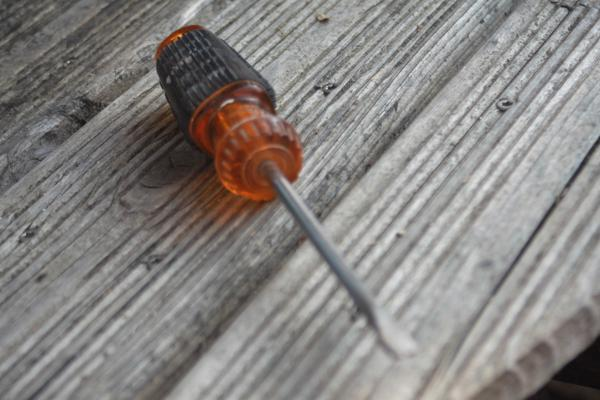
\includegraphics[width=\textwidth]{img/screwdriver1}
	\end{subfigure}
	\hfill
	\begin{subfigure}[b]{0.45\textwidth}
		\centering
		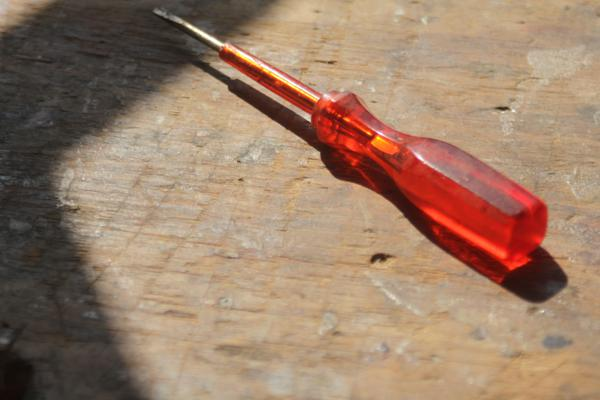
\includegraphics[width=\textwidth]{img/screwdriver2}
	\end{subfigure}
	\caption{Two Images from the TIC Dataset of Class Screwdriver (own figure)}
	\label{fig:screwdriver}
\end{figure}
The dataset is split into a training, validation, and test dataset. For each class, $60\%$ of the images are randomly split for the training dataset, $20\%$ for the validation dataset, and $20\%$ for the test dataset. The resulting training dataset contains $12{,}240$, the resulting validation dataset contains $4{,}080$, and the resulting test dataset contains $4{,}080$ images. For each of these datasets, the images are evenly distributed over all classes.
The training dataset is used to train a neural network. The validation dataset and the test dataset are not used for training. On that account, the neural network cannot overfit to the validation dataset and the test dataset. Thus, the validation dataset can be used to explore different hyperparameters and monitor whether or not the neural network overfits to the training dataset. Based on the performance on the validation dataset, the neural network is chosen for evaluation. This way, the neural network might develop a dependency on the validation dataset. For example, a neural network might perform well on the validation dataset by chance but less well on other data. For this reason, the neural network is evaluated only once on the test dataset. The performance of  the neural network on the test dataset is regarded as the performance of the neural network. \autocite{ElAmir.2020}



\subsection{Neural Network Selection}
To determine the best-performing neural network for tool image classification, optimally, this paper would conduct a neural network architecture search and hyperparameter search. However, resources and time of this paper are limited. Due to that, conducting a neural network architecture search and hyperparameter search is not possible. 
\par
Tool image classification is a sub-task of image classification. Therefore, this paper selects the state-of-the-art neural networks for image classification to conduct the experiment. The state-of-the-art neural networks for image classification are determined as described in Section \ref{sec:litrev}. For each selected neural network the network architecture and the hyperparameters are adopted from the paper originally proposing the neural network. The following neural networks are selected to conduct the experiment:
\begin{itemize}
	\item VGG-19, see Section \ref{sec:conv}. \autocite{Simonyan.2014}
	\item ResNet-152, see Section \ref{sec:res}. \autocite{He.2016}
	\item ResNext-101, see Section \ref{sec:inception}. \autocite{Xie.2017}
	\item DenseNet-264, see Section \ref{sec:dense}. \autocite{Huang.2017}
	\item EfficientNet-B7, see Section \ref{sec:sepconv}. \autocite{Tan.2019}
\end{itemize}
This paper implements the selected neural networks based on their Keras implementation.\autocite{KerasApp} Note that CapsNet is excluded since it does not reach state-of-the-art performance on image classification except for classification of digits or letters.



\subsection{Training}% Training Hyperparams
The neural networks are trained on the training dataset and their performance is monitored on the validation dataset.
Training is carried out by optimizing the categorical cross entropy loss function \autocites{Michelucci.2019}{ElAmir.2020}{Singh.2020}, see Section \ref{sec:training}. Each selected neural network is trained with the number of epochs, the optimizer, and the hyperparameters of the optimizer as specified in the paper originally proposing the neural network.
The hyperparameters of the optimizer are initial learning rate, learning rate schedule, and momentum or Nesterove momentum if used. The learning rate schedule determines how the learning rate changes with epochs progressing.
The batch size specified in the original papers are powers of 2. However, those batch sizes are too large to fit the available GPU. Therefore, the power is reduced by one until the batch size fits the available GPU. For each neural network, the training hyperparameters, namely number of epochs, the optimizer, the hyperparameters of the optimizer, and the batch size are displayed in Table \ref{tab:hyperparams}. \autocites{Simonyan.2014}{He.2016}{Xie.2017}{Huang.2017}{Tan.2019}
\par
For EfficientNet-B7, the number of epochs is not specified, instead EfficientNet-B7 is trained until convergence. \autocite{Tan.2019} The available $200$ hours on the provided hardware might not be enough to train EfficientNet-B7 until convergence. Therefore, the other neural networks are trained before EfficientNet-B7. EfficientNet-B7 is trained for the remaining time.
\begin{xltabular}{\textwidth}{llX}\toprule
	\caption[Training Hyperparameters]{Training Hyperparameters \autocites{Simonyan.2014}{He.2016}{Xie.2017}{Huang.2017}{Tan.2019}} \label{tab:hyperparams}\\
	\textbf{Neural Network} & \textbf{Training Hyperparameters} & \\\midrule \endhead
	VGG-19 & Epochs: & $74$\\
		& Optimizer: & \ac{SGD}\\
		& Initial Learning Rate: & $0.01$\\
		& Learning Rate Schedule: & divide learning rate by $10$ on accuracy plateaus.\\
		& Momentum: & $0.9$\\
		& Batch Size: & $32$\\
	\\\midrule
	ResNet-152 & Epochs: & $120$\\
		& Optimizer: & \ac{SGD}\\
		& Initial Learning Rate: & $0.1$\\
		& Learning Rate Schedule: & divide learning rate by $10$ on accuracy plateaus.\\
		& Momentum: & $0.9$\\ 
		& Batch Size: & $32$\\
	\\\midrule
	ResNeXt-101 & Epochs: & $120$\\
		& Optimizer: & \ac{SGD}\\
		& Initial Learning Rate: & $0.1$\\
		& Learning Rate Schedule: & divide learning rate by $10$ at epoch $30$, $60$, and $90$.\\
		& Momentum: & $0.9$\\ 
		& Batch Size: & $16$\\
	\\\midrule
	DenseNet-264 & Epochs: & $90$\\
		& Optimizer: & \ac{SGD}\\
		& Initial Learning Rate: & $0.1$\\
		& Learning Rate Schedule: & divide learning rate by $10$ at epoch $30$ and $60$.\\
		& Nesterov Momentum: & $0.9$\\
		& Batch Size: & $32$\\
	\\\midrule
	EfficientNet-B7 & Epochs: & not specified\\
		& Optimizer: & \ac{RMSProp}\\
		& Initial Learning Rate: & $0.256$\\
		& Learning Rate Schedule: & decay learning rate by $0.97$ each $2.4$ epochs.\\
		& Momentum: & $0.9$\\
		& Batch Size: & $1$
	\\\bottomrule
\end{xltabular}
Note that metalearning, semi- or unsupervised learning, transfer learning, adversarial training, data augmentation, input normalization, weight decay, and multi-task learning are excluded from the scope of this paper,  see Section \ref{sec:scope}. In consequence, they are excluded from the experiment even if they are used in the original papers.

\subsection{Evaluation}
As mentioned, during training the performance of each neural network is monitored on the validation dataset. The performance is measured at the end of each epoch. After training for the entire number of epochs, the neural network from the epoch with the highest performance is evaluated. A neural network is evaluated on the test dataset. The resulting performance measured in accuracy is reported in Chapter \ref{chp:result}.

\chapter{State of the Art}
\label{ch:sota}
	Over the years the research community has introduced various neural models for text classification.\autocites{Yang.2016}{Cho.2014}{Lee.2016}{Hochreiter.1997}{Kant.2018}{Zhou.2016}{Wang.2016}{Liang.2019}{Kim.2014}{Gao.2018}{Zhang.2015}{Johnson.2017}{Hoa.2017}{Yang.2018}{Rezaeinia.2018}{Zhao.2018}{Lai.2015}{Zheng.2019}{Johnson.2016}{Vaswani.2017}{Wang.2018b}{Iyyer.2015} In order to capture the whole variety of neural text classification models leaderboards, journals and academic full text databases have been screened for papers on neural text classification, namely:
	\begin{itemize}
		\item Association for Computational Linguistics \footnote{\url{https://www.aclweb.org/portal/}}
		\item Institute of Electrical and Electronics Engineers Xplore \footnote{\url{https://ieeexplore.ieee.org/Xplore/home.jsp}}
		\item Association for Computing Machinery Digital Library \footnote{\url{https://dl.acm.org/}}
		\item arXiv\footnote{\url{https://arxiv.org/}}
		\item Journal of Machine Learning Research\footnote{\url{http://www.jmlr.org/}}
		\item MIT Press Journals\footnote{\url{http://proceedings.mlr.press/}}
		\item Proceedings of Machine Learning Research\footnote{\url{http://proceedings.mlr.press/}}
		\item Papers With Code\footnote{\url{https://paperswithcode.com/}}
		\item GLUE\footnote{\url{https://gluebenchmark.com/leaderboard/}}
		\item NLP-Progress\footnote{\url{https://nlpprogress.com/}}
		\item Open AI\footnote{\url{https://openai.com/}}
		\item Google Scholar \footnote{\url{https://scholar.google.de/}}
	\end{itemize}
	The papers have been queried from these databases based on search queries created from Term Table \ref{tab:term_table} and selected based on the selection criteria listed in Section \ref{sec:selection_criteria}. Due to time constraints, this paper leaves out some databases, like Open Review\footnote{\url{https://openreview.net/}}. Nevertheless, this paper has analyzed over 100 papers on neural text classification. On that account, it is very likely all frequently used models are captured. The most used models are listed in Concept Matrix \ref{tab:concept_matrix} and described in this chapter. The concept matrix maps literature to the models they support. The remaining models are listed in Section \ref{sec:misc}.

	\section{\ac{CNN}}
		A highly regarded \ac{CNN} is the LeNet5 by Yann LeCun. LeNet5 was originally used for image classification. A grayscale image can be represented as matrix with each element corresponding to the grayscale of a pixel. Colored images can be represented in the same way by three matrices one for the red, green and blue scale value of a pixel. These matrices are called channels. A \ac{CNN} is structured like a \ac{MLP}, which neurons only connect partially to the input, see Figure \ref{img:cnn:neuron}. \autocite{LeCun.1998}
		\begin{figure}[H]
			\centering
			\begin{tikzpicture}
				\node[draw, circle, minimum size=1.2cm] (n) at (5,2.8) {};
				\draw (n) --  (7,2.8);
				\foreach \x in {0,1,2,3,4}
					\foreach \y in {0,1,2,3,4}
						\draw (\x*0.9+ \y*0, \x*0.4+\y*1) circle (0.2cm); %Matrixtransformation (0.7 0; 0.3 1)
				\foreach \x in {1,2,3}
					\foreach \y in {1,2,3} {
						\draw (\x*0.9+ \y*0, \x*0.4+\y*1) -- (n);
						\fill (\x*0.9+ \y*0, \x*0.4+\y*1) circle (0.1cm);
					}
			\end{tikzpicture}
			\caption{Neuron of a \ac{CNN} (own figure)} \label{img:cnn:neuron}
		\end{figure}
		In order to understand a \ac{CNN} three main operations need to be explained:
		\begin{itemize}
			\item Convolution
			\item Non Linearity
			\item Sub-Sampling
		\end{itemize}
		\paragraph{Convolution} in regard to \ac{CNN}s loosely refers to discrete convolution. Let the input matrix be $X$. Further, let the weight matrix of the \ac{CNN}'s neuron be $w$ with $k$ rows and $l$ columns called filter or kernel. Further, let the sub matrix resulting from the area the neuron is connected to be $X[i:i+l-1, j:j+k-1]$. Then the convolution is defined as \eqref{eq:convolution}.
			\begin{equation}
				\label{eq:convolution}
				X * w := w \cdot X[i:i+l-1, j:j+k-1] = O
			\end{equation}
		Meaning that each element of the resulting output matrix $O$ is the matrix product between the sub matrix of the area the neuron is connected to and the weight matrix of the neuron. The factor by which $i$ and $j$ are incremented determines the area the neuron is connected to. This factor is called $stride$. In consequence, an output matrix is produced for each kernel. The resulting output matrices are called activation maps or feature maps. \autocite{Zhang.2015c}
		\par
		In order to illustrate this abstract definition, consider the case of a grayscale image represented as a matrix $X$, as shown in Figure \ref{img:conv}. Furthermore, consider the kernel $w$, as shown in Figure \ref{img:conv}. Then, the convolution of the image and the kernel can be computed by laying the kernel on top of the image. The element of the activation map is computed by multiplying and summing the overlapping elements. To iterate through the elements the kernel is \enquote{slid} over each row and each column. Resulting in the output $O$, as shown in Figure \ref{img:conv}.
		\begin{figure}[H]
			\centering
			\begin{tikzpicture}
			\matrix (mtr) [matrix of nodes,row sep=-\pgflinewidth, nodes={draw}]
			{
				0 & 1 & 0 & |[fill=orange!30]| 1 & |[fill=orange!30]| 0 & |[fill=orange!30]| 0 & 0 & 0 & 0\\
				0 & 0 & 1 & |[fill=orange!30]| 1 & |[fill=orange!30]| 1 & |[fill=orange!30]| 0 & 0 & 1 & 0\\
				1 & 0 & 0 & |[fill=orange!30]| 1 & |[fill=orange!30]| 1 & |[fill=orange!30]| 1 & 0 & 1 & 0\\
				0 & 0 & 0 & 0 & 1 & 0 & 0 & 0 & 0\\
				0 & 0 & 1 & 1 & 0 & 1 & 0 & 0 & 1\\
				0 & 1 & 1 & 1 & 0 & 1 & 1 & 0 & 1\\
				0 & 1 & 1 & 0 & 0 & 0 & 1 & 1 & 0\\
			};
			
			\draw[very thick, orange] (mtr-1-4.north west) rectangle (mtr-3-6.south east);
			
			\node [below= of mtr-5-5.south] (lm) {$X$};
			
			\node[right = 0.2em of mtr] (str) {$\cdot$};
			
			\matrix (K) [right=0.2em of str,matrix of nodes,row sep=-\pgflinewidth, nodes={draw, fill=blue!30}]
			{
				1 & 0 & 1 \\
				0 & 1 & 0 \\
				1 & 0 & 1 \\
			};
			\node [below = of K-3-2.south] (lk) {$K$};
			
			\node [right = 0.2em of K] (eq) {$=$};
			
			\matrix (ret) [right=0.2em of eq,matrix of nodes,row sep=-\pgflinewidth, nodes={draw}]
			{
				1 & 4 & 2 & |[fill=black!30!green!30]| 4 & 1 & 2 & 1\\
				1 & 1 & 4 & 2 & 3 & 1 & 1\\
				2 & 2 & 2 & 5 & 1 & 3 & 1\\
				1 & 3 & 3 & 2 & 3 & 1 & 2\\
				3 & 3 & 2 & 2 & 2 & 3 & 2\\
			};
			\node [below = of ret-4-4.south] (lim) {$Y = \varphi(\sum X[i:i+k, j:j+k] \cdot K$};
			
			\draw[very thick, black!30!green] (ret-1-4.north west) rectangle (ret-1-4.south east);
			
			\draw[densely dotted, blue, thick] (mtr-1-4.north west) -- (K-1-1.north west);
			\draw[densely dotted, blue, thick] (mtr-3-4.south west) -- (K-3-1.south west);
			\draw[densely dotted, blue, thick] (mtr-1-6.north east) -- (K-1-3.north east);
			\draw[densely dotted, blue, thick] (mtr-3-6.south east) -- (K-3-3.south east);
			
			\draw[densely dotted, black!30!green, thick] (ret-1-4.north west) -- (K-1-1.north west);
			\draw[densely dotted, black!30!green, thick] (ret-1-4.south west) -- (K-3-1.south west);
			\draw[densely dotted, black!30!green, thick] (ret-1-4.north east) -- (K-1-3.north east);
			\draw[densely dotted, black!30!green, thick] (ret-1-4.south east) -- (K-3-3.south east);
			
			\matrix (K) [right=0.2em of str,matrix of nodes,row sep=-\pgflinewidth, nodes={draw, fill=blue!10}]
			{
				1 & 0 & 1 \\
				0 & 1 & 0 \\
				1 & 0 & 1 \\
			};
			
			\draw[very thick, blue] (K-1-1.north west) rectangle (K-3-3.south east);
			
			\node[anchor=south east, inner sep=0.01em, blue] at (mtr-1-4.south east) (xx) {\scalebox{.5}{$\times 1$}};
			\node[anchor=south east, inner sep=0.01em, blue] at (mtr-1-5.south east) (xx) {\scalebox{.5}{$\times 0$}};
			\node[anchor=south east, inner sep=0.01em, blue] at (mtr-1-6.south east) (xx) {\scalebox{.5}{$\times 1$}};
			\node[anchor=south east, inner sep=0.01em, blue] at (mtr-2-4.south east) (xx) {\scalebox{.5}{$\times 0$}};
			\node[anchor=south east, inner sep=0.01em, blue] at (mtr-2-5.south east) (xx) {\scalebox{.5}{$\times 1$}};
			\node[anchor=south east, inner sep=0.01em, blue] at (mtr-2-6.south east) (xx) {\scalebox{.5}{$\times 0$}};
			\node[anchor=south east, inner sep=0.01em, blue] at (mtr-3-4.south east) (xx) {\scalebox{.5}{$\times 1$}};
			\node[anchor=south east, inner sep=0.01em, blue] at (mtr-3-5.south east) (xx) {\scalebox{.5}{$\times 0$}};
			\node[anchor=south east, inner sep=0.01em, blue] at (mtr-3-6.south east) (xx) {\scalebox{.5}{$\times 1$}};
			
			\end{tikzpicture}
			\caption{Convolution Illustration (own figure)} \label{img:conv}
		\end{figure}
		As shown in Figure \ref{img:conv}, the resulting output is smaller than the original input. To preserve the original size, $padding$ may be used. $Padding$ can be described as adding zeros at the edges of the input. Therefore, the output size results in Equation \eqref{eq:conv:output}.\autocite{Conneau.2016}
		\begin{equation}
			output size = \frac{input size - kernel size + 2 \cdot padding}{stride} + 1
			\label{eq:conv:output}
		\end{equation}
		\paragraph{Non linearity} needs to be applied to the convolution in order to model non linearly correlated data, because the convolution as defined in \eqref{eq:convolution} is completely linear. Applying a non linear activation function $\varphi$ and a bias $b$ results in Equation \eqref{eq:conv:neuron}.\autocite{LeCun.1998}
		\begin{equation}
			y = \varphi(X * w + b) = \varphi(w \cdot X[i:i+l-1, j:j+k-1] + b)
			\label{eq:conv:neuron}
		\end{equation}
		Thus, Equation \eqref{eq:conv:neuron} is rather similar to Equation \eqref{eq:neuron:y} which is used in Section \ref{sec:neuron} to describe a neuron. The only difference is the shape of the input the neuron is connected to. Deducing from this, neurons of a \ac{MLP} and a \ac{CNN} do not differ in their structure.
		\paragraph{Sub-sampling} is used after convolution and non linearity are applied. \autocite{LeCun.1998} Sub-sampling means reducing the size of the feature maps. The computational complexity of a \ac{CNN} increases over depth in regard to the number and size of the feature maps.\autocites{Conneau.2016}{Johnson.2017} Due to that, sub-sampling reduces the computational complexity in multi layer \ac{CNN}s. Sub-sampling can be achieved by different strategies. However, \cite{Zhang.2015c} found that max pooling outperforms other sub-sampling strategies. Max pooling is defined as \eqref{eq:maxp}.\autocite{Boureau.2010}
		\begin{equation}
			\label{eq:maxp}
			MaxPooling(X) := max(X[i:i+l-1, j:j+k-1])
		\end{equation}
		Accordingly, max pooling works similar to convolution. The pooling kernel is \enquote{slid} over the input matrix, but instead of convolving the sub matrix and the filter, the maximum of the sub matrix is taken, see Figure \ref{img:maxp}.
		\begin{figure}[H]
			\centering
			\begin{tikzpicture}
			\matrix (mtr) [matrix of nodes,row sep=-\pgflinewidth, nodes={draw}]
			{
				0 & 1 & 0 & |[fill=orange!30]| 1 & |[fill=orange!30]| 0 & |[fill=orange!30]| 0 & 0 & 0 & 0\\
				0 & 0 & 4 & |[fill=orange!30]| 1 & |[fill=orange!30]| 2 & |[fill=orange!30]| 0 & 0 & 1 & 0\\
				2 & 0 & 0 & |[fill=orange!30]| 1 & |[fill=orange!30]| 4 & |[fill=orange!30]| 1 & 0 & 1 & 0\\
				0 & 0 & 0 & 0 & 1 & 0 & 3 & 0 & 0\\
				0 & 0 & 1 & 1 & 0 & 1 & 0 & 0 & 0\\
				0 & 1 & 1 & 3 & 0 & 1 & 0 & 0 & 0\\
				0 & 1 & 1 & 0 & 0 & 0 & 1 & 1 & 0\\
			};
			
			\draw[very thick, orange] (mtr-1-4.north west) rectangle (mtr-3-6.south east);
			
			\node [below= of mtr-5-5.south] (lm) {$\bf X$};
			
			\node [below = of K-3-2.south] (lk) {$\bf Kernel$};
			
			\matrix (ret) [right=0.2em of eq,matrix of nodes,row sep=-\pgflinewidth, nodes={draw}]
			{
				4 & 4 & 4 & |[fill=black!30!green!30]| 4 & 4 & 1 & 1\\
				4 & 4 & 4 & 4 & 4 & 3 & 3\\
				2 & 1 & 4 & 4 & 4 & 3 & 3\\
				1 & 3 & 3 & 3 & 3 & 3 & 3\\
				1 & 3 & 3 & 3 & 1 & 1 & 1\\
			};
			\node [below = of ret-4-4.south] (lim) {${\bf MaxPooling(X)}$};
			
			\draw[very thick, black!30!green] (ret-1-4.north west) rectangle (ret-1-4.south east);
			
			\draw[densely dotted, blue, thick] (mtr-1-4.north west) -- (K-1-1.north west);
			\draw[densely dotted, blue, thick] (mtr-3-4.south west) -- (K-3-1.south west);
			\draw[densely dotted, blue, thick] (mtr-1-6.north east) -- (K-1-3.north east);
			\draw[densely dotted, blue, thick] (mtr-3-6.south east) -- (K-3-3.south east);
			
			\draw[densely dotted, black!30!green, thick] (ret-1-4.north west) -- (K-1-1.north west);
			\draw[densely dotted, black!30!green, thick] (ret-1-4.south west) -- (K-3-1.south west);
			\draw[densely dotted, black!30!green, thick] (ret-1-4.north east) -- (K-1-3.north east);
			\draw[densely dotted, black!30!green, thick] (ret-1-4.south east) -- (K-3-3.south east);
			
			\matrix (K) [right=0.2em of str,matrix of nodes,row sep=-\pgflinewidth, nodes={draw, fill=blue!10}]
			{
				 &  & \\
				 &  & \\
				 &  & \\
			};
			
			\draw[very thick, blue] (K-1-1.north west) rectangle (K-3-3.south east);
			
			\end{tikzpicture}
			\caption{Max Pooling Illustration (own figure)} \label{img:maxp}
		\end{figure}
		\par
		These three operations form the basic building block of a \ac{CNN}. This building block is comprised of a convolutional layer followed by a non linearity. The pooling layer is applied after the non linearity and is optional. This building block can be repeated any number of times. \autocite{LeCun.1998} This is illustrated in Figure \ref{img:cnn}.
		\begin{figure}[H]
			\centering
			\begin{tikzpicture}
	\begin{scope}[yslant=1,xshift=0.2]
		\foreach \i in {0,0.1,0.2}
			\draw [fill=lightgray] (0+\i,0-\i) rectangle (4+\i,4-\i);
		
		\foreach \i in {0,0.1,0.2,0.3,0.4,0.5}
			\draw [fill=lightgray] (5+\i,-5-\i) rectangle (8+\i,-2-\i);
			
		\foreach \i in {0,0.1,0.2,0.3,0.4,0.5}
			\draw [fill=lightgray] (8.5+\i,-8.5-\i) rectangle (10.5+\i,-6.5-\i);
			
		\foreach \i in {0,0.1,0.2,0.3,0.4,0.5}
			\draw [fill=lightgray] (11.5+\i,-11.5-\i) rectangle (12+\i,-11-\i);
		
		\draw [thick, blue] (1,1) rectangle (2.5,2.5);
		\draw [thick, blue] (6,-4) rectangle (6.5,-3.5);
		\draw[densely dotted, blue, thick] (1,1) -- (6,-4);
		\draw[densely dotted, blue, thick] (1,2.5) -- (6,-3.5);
		\draw[densely dotted, blue, thick] (2.5,1) -- (6.5,-4);
		\draw[densely dotted, blue, thick] (2.5,2.5) -- (6.5,-3.5);
		
		\draw [thick, orange] (7,-4) rectangle (8,-3);
		\draw [thick, orange] (10.5,-8) rectangle (11,-8.5);
		\draw[densely dotted, orange, thick] (7,-4) -- (10.5,-8.5);
		\draw[densely dotted, orange, thick] (7,-3) -- (10.5,-8);
		\draw[densely dotted, orange, thick] (8,-4) -- (11,-8.5);
		\draw[densely dotted, orange, thick] (8,-3) -- (11,-8);
		
		\draw [thick, blue] (9,-9) rectangle (11,-7);
		\draw [thick, blue] (12,-12) rectangle (12.5,-11.5);
		\draw[densely dotted, blue, thick] (9,-9) -- (12,-12);
		\draw[densely dotted, blue, thick] (9,-7) -- (12,-11.5);
		\draw[densely dotted, blue, thick] (11,-9) -- (12.5,-12);
		\draw[densely dotted, blue, thick] (11,-7) -- (12.5,-11.5);
	\end{scope}
	
	\node (in) at (0,-0.5) {3 input channels};
	\node (h1) at (4,-0.5) {6 activation maps};
	\node (h2) at (7.7,-0.5) {6 activation maps};
	\node (out) at (11.5,-0.5) {6 activation maps};
	
	\node [text=blue, align=left,text width=10em] (conv) at (0,7.5) {\bf Convolution+ReLu};
	\node [text=orange, align=left,text width=10em] (pool) at (0,6.5) {\bf Max Pooling};
\end{tikzpicture}
			\caption{\ac{CNN} (own figure)} \label{img:cnn}
		\end{figure}
	\paragraph{For text classification} the \ac{CNN} works in the same way. The input for text classification can be described as a sequence of words. These words can be embedded as vectors which are concatenated into a sequence matrix. This sequence matrix is the input channel to the \ac{CNN}.\autocite{Kim.2014}
		
	\section{\ac{RNN}}
		A \ac{RNN} is structured like a \ac{MLP} with neurons connect to themselves, see Figure \ref{img:rnn}. \autocite{Elman.1990} Due to that, the output of a \ac{RNN}, in contrast to a \ac{MLP}, is dependent on previous computations. On this account, \ac{RNN}s are able to process sequential information like text. A text can be seen as a sequence of words. These words can be encoded as vectors. \autocites{Wang.2012}{Turian.2010}{Mikolov.2013}{Mikolov.2013b}{Joulin.2016}{Smith.2019}{Pennington.2014}{McCann.2017} This results in a sequence of vectors. Each element of that sequence is processed in the same way. That is why \ac{RNN}s are called recurrent. 
		\begin{figure}[H]
			\centering
			\begin{tikzpicture}[-latex,auto,node distance=2cm,thick]
	
	\node [draw, circle, minimum size=0.9cm,blue] (A) at (0,0) {$x_0$};
	\node [draw, circle, minimum size=0.9cm,orange] (B) [right of=A] {};
	\node [draw, circle, minimum size=0.9cm,black!30!green] (C) [right of=B] {$h_0$};
	
	\node [draw, circle, minimum size=0.9cm,blue] (D) [below of=A] {$x_1$};
	\node [draw, circle, minimum size=0.9cm,orange] (E) [right of=D] {};
	\node [draw, circle, minimum size=0.9cm,black!30!green] (F) [right of=E] {$h_1$};
	
	\node [draw, circle, minimum size=0.9cm,blue] (G) [below of=D] {$x_2$};
	\node [draw, circle, minimum size=0.9cm,orange] (H) [right of=G] {};
	\node [draw, circle, minimum size=0.9cm,black!30!green] (I) [right of=H] {$h_2$};
	
	\path (A) edge (B) (B)	edge (C) (B) edge [loop above] (B)
		(D) edge (E) (E)	edge (F) (E) edge [loop above] (E)
		(G) edge (H) (H)	edge (I) (H) edge [loop above] (H)
		(B) edge [bend left] (E) (E)	edge [bend left] (H)
		(H) edge [bend left] (E) (E)	edge [bend left] (B)
		(A) edge (E) (A) edge (H) (D) edge (B) (D) edge (H) (G) edge (B) (G) edge (E);
\end{tikzpicture}
			\caption{Recurrent Neural Network (own figure)} \label{img:rnn}
		\end{figure}
		As shown in Section \ref{sec:mlp}, connections can be described using a weight matrix. Therefore, let the recurrent connections be described by the weight matrix $W^{(hh)}$ and the connections to the input by the weight matrix $W^{(hx)}$. Further let the input vector $x_t$ be element of the  sequence $(x_1, x_2 \dots x_n)$. Then the information, carried between each time step $t$ of the sequence, called hidden state $h_t$, can be described as \eqref{eq:rnn:hiddenstate}.
		\begin{equation}
			h_t = \varphi(W^{(hh)}h_{t-1}+W^{(hx)}x_t)
			\label{eq:rnn:hiddenstate}
		\end{equation}
		Consequently, in theory \ac{RNN}s are able to propagate information through arbitrarily long sequences. However, in practice they are limited to only a few time steps. This is because of the vanishing gradient problem. \autocite{Hochreiter.2001} In order to overcome the vanishing gradient problem \ac{LSTM} \autocite{Hochreiter.1997} and \ac{GRU} \autocite{Cho.2014} were designed. Both variations use gated units and a memory vector to directly propagate information between time steps, thus preventing the information from vanishing. \autocite{Hochreiter.2001} According to the results of the papers reviewed for the Concept Matrix \ref{tab:concept_matrix}, both variations perform much better than vanilla \ac{RNN}s. However, neither \ac{GRU}s, nor \ac{LSTM}s seem to have a significant performance advantage over the other.\autocites{Greff.2015}{Shah.2015} As more of the reviewed papers used \ac{LSTM}s, this paper only introduces \ac{LSTM}s. A \ac{LSTM} consists of one \ac{LSTM} cell per time step in a sequence.
		A \ac{LSTM} cell at time step $t$ consists of an input gate $i_t$, an output gate $o_t$, a forget gate $f_t$ and a cell state $c_t$, see Figure \ref{img:lstm}. The cell state runs along the entire sequence only influenced by information filtered through the input and forget gate. Therefore, information can be preserved over a long sequence.
		Gates use the sigmoid function $\sigma$ and element wise multiplication $\otimes$ to block or convey information. The sigmoid function \enquote{squashes} all values in the range of $[0;1]$,  thus creating a vector which scalars are in the range of $[0;1]$. Any scalar multiplied by $0$ is $0$. Due to that, any information conveyed by that scalar is blocked. Accordingly, any multiplier above $0$ conveys a portion of the information. In consequence, the element wise multiplication multiplies all scalars with a scalar in range of $[0;1]$.
		The forget gate applies this operations to the cell state. The scalars of the cell state multiplied by $0$ are \enquote{forgotten}. The input gate applies a non linearity to the input information, and uses the gating mechanism to decide what part of that information is added to the cell state. The resulting information is called new cell content $\tilde{c_t}$. The output gate applies a non linearity to the cell state, and uses the information conveyed by the input gate for its own gating mechanism to decide what information of the cell state is returned as output. The output is called hidden state $h_t$.
		\begin{figure}[H]
			\centering
			% Code mostly compypasted from By J. Leon, Beerware licence is acceptable..., under https://tex.stackexchange.com/questions/432312/how-do-i-draw-an-lstm-cell-in-tikz

\begin{tikzpicture}[
	% GLOBAL CFG
	font=\sf \scriptsize,
	>=LaTeX,
	% Styles
	cell/.style={% For the main box
		rectangle, 
		rounded corners=5mm, 
		draw,
		very thick,
	},
	operator/.style={%For operators like +  and  x
		circle,
		draw,
		inner sep=-0.5pt,
		minimum height =.2cm,
	},
	function/.style={%For functions
		ellipse,
		draw,
		inner sep=1pt
	},
	ct/.style={% For external inputs and outputs
		circle,
		draw,
		line width = .75pt,
		minimum width=1cm,
		inner sep=1pt,
	},
	gt/.style={% For internal inputs
		rectangle,
		draw,
		minimum width=4mm,
		minimum height=3mm,
		inner sep=1pt
	},
	mylabel/.style={% something new that I have learned
		font=\scriptsize\sffamily, 
		align=center,
	},
	ArrowC1/.style={% Arrows with rounded corners
		rounded corners=.25cm,
		thick,
	},
	ArrowC2/.style={% Arrows with big rounded corners
		rounded corners=.5cm,
		thick,
	},
	]
	
	%Start drawing the thing...  
	\draw[orange, fill=orange!30,rounded corners=5mm] (-3,-2) rectangle (-1.77,2);
	\draw[blue, fill=blue!30,rounded corners=5mm] (-1.75,-2) rectangle (0.18,1);
	\draw[black!30!green, fill=black!30!green!30,rounded corners=5mm] (0.2,-2) rectangle (2.25,1.25);
	\node[orange] (f) at (-5,0) {\bf \large forget gate};
	\node[blue] (i) at (0,-3) {\bf \large input gate};
	\node[black!30!green] (o) at (5,0) {\bf \large output gate};
	% Draw the cell: 
	\node [cell, minimum height =4cm, minimum width=6cm] at (0,0){} ;
	
	% Draw inputs named ibox#
	\node [gt] (ibox1) at (-2,-0.75) {$\sigma$};
	\node [gt] (ibox2) at (-1.5,-0.75) {$\sigma$};
	\node [gt, minimum width=1cm] (ibox3) at (-0.5,-0.75) {Tanh};
	\node [gt] (ibox4) at (0.5,-0.75) {$\sigma$};
	
	% Draw opérators   named mux# , add# and func#
	\node [operator] (mux1) at (-2,1.5) {$\times$};
	\node [operator] (add1) at (-0.5,1.5) {+};
	\node [operator] (mux2) at (-0.5,0) {$\times$};
	\node [operator] (mux3) at (1.5,0) {$\times$};
	\node [function] (func1) at (1.5,0.75) {Tanh};
	
	% Draw External inputs? named as basis c,h,x
	\node[ct, label={[mylabel]Previous \\ Cell State}] (c) at (-4,1.5) {$c_{t-1}$};
	\node[ct, label={[mylabel]Previous \\ Hidden State}] (h) at (-4,-1.5) {$h_{t-1}$};
	\node[ct, label={[mylabel]left:Input}] (x) at (-2.5,-3) {$x_t$};
	
	% Draw External outputs? named as basis c2,h2,x2
	\node[ct, label={[mylabel]Cell State}] (c2) at (4,1.5) {$c_t$};
	\node[ct, label={[mylabel]Hidden State}] (h2) at (4,-1.5) {$h_t$};
	\node[ct, label={[mylabel]left:Hidden State}] (x2) at (2.5,3) {$h_t$};
	
	% Start connecting all.
	%Intersections and displacements are used. 
	% Drawing arrows    
	\draw [ArrowC1] (c) -- (mux1) -- (add1) -- (c2);
	\draw [ArrowC1] (c) -- (-2.5, 1.5) -- (-2.5, -1.5) -- (-2, -1.5) -- (ibox1);
	
	% Inputs
	\draw [ArrowC2] (h) -| (ibox4);
	\draw [ArrowC1] (h -| ibox1)++(-0.5,0) -| (ibox1); 
	\draw [ArrowC1] (h -| ibox2)++(-0.5,0) -| (ibox2);
	\draw [ArrowC1] (h -| ibox3)++(-0.5,0) -| (ibox3);
	\draw [ArrowC1] (x) -- (x |- h)-| (ibox3);
	
	% Internal
	\draw [-latex, ArrowC2] (ibox1) -- (mux1);
	\draw [-latex, ArrowC2] (ibox2) |- (mux2);
	\draw [-latex, ArrowC2] (ibox3) -- (mux2);
	\draw [-latex, ArrowC2] (ibox4) |- (mux3);
	\draw [-latex, ArrowC2] (mux2) -- (add1);
	\draw [-latex, ArrowC1] (add1 -| func1)++(-0.5,0) -| (func1);
	\draw [-latex, ArrowC2] (func1) -- (mux3);
	
	%Outputs
	\draw [-, ArrowC2] (mux3) |- (h2);
	\draw (c2 -| x2) ++(0,-0.1) coordinate (i1);
	\draw [-, ArrowC2] (h2 -| x2)++(-0.5,0) -| (i1);
	\draw [-, ArrowC2] (i1)++(0,0.2) -- (x2);

\end{tikzpicture}
			\caption{LSTM Cell (based on \cite{Graves.2013})} \label{img:lstm}
		\end{figure}
		As described so far, the gates do not know what information to block or convey. That is why \ac{MLP}s are used inside the gates, having either $Tanh$ or $\sigma$ as their activation function. These \ac{MLP}s learn to operate the gates. They consist of an input layer, an output layer and one hidden layer. As shown in Section \ref{sec:mlp}, these layers can be described by matrices, denoted $W$. In consequence, a \ac{LSTM} can be described as in Equation \eqref{eq:lstm}. \autocite{Graves.2013} 
		\footnote{As Figure \ref{img:lstm} shows a concatenation while Equation \eqref{eq:lstm} uses a sum operation, it is reasonable to point out that these are equal. $[x_t; h_{t-1}; c_{t-1}] \dot [W_x; W_h; W_c] = x_tW_h + h_{t-1}W_h + c_{t-1}tW_c$}
		\begin{equation}
			\label{eq:lstm}
			\begin{array}{lcl}
				i_t & = & \sigma(W_{xi}x_t + W_{hi}h_{t-1} + W_{ci}c_{t-1} + b_i) \\
				o_t & = & \sigma(W_{xo}x_t + W_{ho}h_{t-1} + W_{co}c_{t-1} + b_o) \\
				f_t & = & \sigma(W_{xf}x_t + W_{hf}h_{t-1} + W_{cf}c_{t-1} + b_f) \\
				\tilde{c_t} & = & Tanh(W_{xc}x_t + W_{hc}h_{t-1} + W_{cc}c_{t-1} + b_c) \\
				c_t & = & i_t \otimes \tilde{c_t} + f_t \otimes c_{t-1} \\
				h_t & = & o_t \otimes Tanh(c_t)
			\end{array}
		\end{equation}
		
	\section{Transformer}
	Architectures based on the Transformer namely BERT \autocite{Devlin.2018}, ALBERT \autocite{Lan.2019} and XLNet \autocite{Yang.2019} dominate the top of the GLUE leaderboard\autocite{Wang.2019}.  \footnote{\url{https://gluebenchmark.com/leaderboard/}} The Transformer, originally introduced by \cite{Vaswani.2017}, mainly utilizes a mechanism called attention. The Transformer is comprised of an encoder and a decoder. However, only the encoder or a modified version of the encoder is used by BERT, ALBERT and XLNet. For this reason, this section focuses on the Transformer encoder. 
	
	The encoder is composed of a stack of $N+1$ Blocks. The first block is comprised of an input embedding and a positional encoder. The remaining $N$ blocks are Transformer blocks. The input to the Transformer encoder is a sequence of words of length $T$. The output of each block is a sequence of hidden states $h_t^{(n)}$ where $t$ is the position in the sequence and $n$ is the block. $n=0$ denotes the first block. As a result, the input of each block is the sequence of previous hidden states. Each block is composed of two layers. The first is a multi-head self-attention mechanism, and the second is a \ac{MLP}. A residual connection\autocite{He.2015}, followed by layer normalization \autocite{Ba.2016} is employed around each of the two layers. Therefore, the output of each layer can be described as in Equation \eqref{eq:transformer}.
	\begin{equation}
		\label{eq:transformer}
		LayerNorm(x + Layer(x))
	\end{equation} 
	With $Layer(x)$ being the function of the layer itself and $LayerNorm(x)$ being the function described by \cite{He.2015}, the residual connections bypass the layers and allow the input to flow past them unchanged. On that account, a residual connection can be described as summing the input vectors to the output vectors. Hence, the inputs and outputs of all layers in the model need to be of the same dimensionality. The Transformer encoder is shown in Figure \ref{img:transformer}.
	\begin{figure}[H]
		\centering
		\begin{tikzpicture}[
	cell/.style={
		rectangle, 
		rounded corners=2mm, 
		draw,
		very thick,
		align=center,
	},
	ArrowC1/.style={% Arrows with rounded corners
		rounded corners=.25cm,
		thick,
	},
	do path picture/.style={%
		path picture={%
			\pgfpointdiff{\pgfpointanchor{path picture bounding box}{south west}}%
			{\pgfpointanchor{path picture bounding box}{north east}}%
			\pgfgetlastxy\x\y%
			\tikzset{x=\x/2,y=\y/2}%
			#1
		}
	},
	sin wave/.style={do path picture={    
			\draw [line cap=round] (-3/4,0)
			sin (-3/8,1/2) cos (0,0) sin (3/8,-1/2) cos (3/4,0);
	}},
]
	\node [cell] (out) at (0,10.5) {Ouput};
	
	\node [cell, fill=lightgray!30, minimum height=6cm, minimum width=5cm, label={[align=center]left:N $\times$ Transformer \\ Block}] (tb) at (-0.25,6.5) {};
	\node [cell, fill=black!30!green!30] (an2) at (0,9) {\textcolor{violet}{Add} \& Norm};
	\node [cell, fill=blue!30] (mlp) at (0,8) {Multi Layer \\ Perceptron};
	\node [cell, fill=black!30!green!30] (an1) at (0,6) {\textcolor{violet}{Add} \& Norm};
	\node [cell, fill=orange!30] (mha) at (0,5) {Multi Head \\ Attention};
	
	
	\node [draw, circle] (+) at (0,2.8) {$+$};
	\node [cell, fill=red!30] (emb) at (0,1.5) {Input \\ Embedding};
	\node [cell] (in) at (0,0) {Input};
	\node[circle, draw, sin wave, minimum size=1.2cm, label={[align=center]left:Positional \\ Encoding}] (pos) at (-2.5,2.8) {};
	
	\draw [-latex,ArrowC1] (in) -- (emb);
	\draw [-latex,ArrowC1] (emb) -- (+);
	\draw [-latex,ArrowC1] (+) -- (0,4) -- (mha);
	\draw [-latex,ArrowC1] (mha) -- (an1);
	\draw [-latex,ArrowC1] (an1) -- (0,7) -- (mlp);
	\draw [-latex,ArrowC1] (mlp) -- (an2);
	\draw [-latex,ArrowC1] (an2) -- (out);
	\draw [-latex, ArrowC1] (pos) -- (+);
	
	\draw [-latex, ArrowC1] (+) -- (0,4) -- (1,4) -- (1,4.5);
	\draw [-latex, ArrowC1] (+) -- (0,4) -- (-1,4) -- (-1,4.5);
	
	\draw [-latex, ArrowC1,violet] (+) -- (0,3.75) -- (-1.75, 3.75) -- (-1.75,3.5 |- an1) node[sloped,above,midway] {Residual} -- (an1);
	\draw [-latex, ArrowC1,violet] (an1) -- (0,7) -- (-1.75, 7) -- (-1.75,7 |- an2) node[sloped,above,midway] {Residual} -- (an2);
\end{tikzpicture}
		\caption{Transformer Encoder (based on \cite{Vaswani.2017})} \label{img:transformer}
	\end{figure}
	\paragraph{Multi-Head Attention} is described in the following paragraph.
	\blockcquote{Vaswani.2017}{An attention function can be described as mapping a query and a set of key-value pairs to an output, where the query, keys, values, and output are all vectors. The output is computed as a weighted sum of the values, where the weight assigned to each value is computed by a compatibility function of the query with the corresponding key.}
	\cite{Vaswani.2017} use dot-product attention \autocite{Bahdanau.2014} scaled by the dimension $d_k$ of the keys. To obtain the scaled dot-product attention the dot-product of the queries with all keys, each divided by $\sqrt{d_k}$ is computed. Subsequently, a softmax function is applied to obtain the weights on the values. At last the values are weighted. The input to a Transformer Block is the sequence of previous hidden states. These hidden states form the queries, the keys and the values. Resulting from this, queries, keys and values are the same, so the attention of a query is to the query itself. For this reason, this kind of attention is called self-attention. In practice, the attention function can be computed on all queries simultaneously, by concatenating the queries into a matrix $Q$, the keys into a matrix $K$ and the values into a matrix $V$, see Equation \eqref{eq:attention}. \autocite{Vaswani.2017}
	\begin{equation}
		\label{eq:attention}
		Attention(Q,K,V)=softmax(\frac{QK^{{\mathrm {T}}}}{\sqrt{d_k}})V
	\end{equation}
	\blockcquote{Vaswani.2017}{Multi-head attention allows the model to jointly attend to information from different representation subspaces at different positions. With a single attention head, averaging inhibits this.}
	Multi-head attention linearly projects the queries, keys and values $h$ times to $d_k$ dimensions. The projection matrices $W_i^Q$, $W_i^K$ and $W_i^V, i \in [1;h]$ are individually learned and thus differ from each other.
	The attention function is applied to each of these projections. The resulting matrices are concatenated and again projected. Resulting in a matrix, being the multi-head attentions output. This is shown in Equation \eqref{eq:multiheadattention}. \autocite{Vaswani.2017}
	\begin{equation}
		\label{eq:multiheadattention}
		\begin{array}{rcl}
			MultiHead(Q,K,V) & = & Concat(head_1, head_2, \dots head_h) W^O \\
			\text{where }head_i & = & Attention(QW_i^Q,KW_i^K,VW_i^V)
		\end{array}
	\end{equation}
	\paragraph{\ac{MLP}s} cannot be applied to matrices. This is a problem, because the multi-head attention, as described in Equation \eqref{eq:multiheadattention} returns a matrix. However, this matrix is comprised of attention vectors. On this account one \ac{MLP} can be applied per attention vector. \autocite{Vaswani.2017}
	\paragraph{Input embeddings} are used to convert tokens to vectors. The input embedding is a learned embedding. This is similar to other embedding approaches, like \cites{Wang.2012}{Turian.2010}{Mikolov.2013}{Mikolov.2013b}{Joulin.2016}{Smith.2019}{Pennington.2014}{McCann.2017}. \autocite{Vaswani.2017}
	\paragraph{Positional Encoding} is used to inject information about a token's relative or absolute position in the input sequence. This is necessary since the attention mechanism, unlike recurrence or convolution, does not preserve spatial information. In order to be summed, positional encoding and input embedding must have the same dimensionality $d$. Each embedded token is a vector of size $d$. Consequently the positional encoding must return a scalar for each dimension $i \in [1,d]$ \autocite{Vaswani.2017}. \cite{Vaswani.2017} uses the sine and cosine functions of different frequencies to encode a token's position $pos$ in the input sequence , as shown in Equation \eqref{eq:posemb}.
	\begin{equation}
		\label{eq:posemb}
		\begin{array}{rcl}
			PositionEmbedding(pos,2i) & = & sin(\frac{pos}{100000^{2 / d}}) \\
			PositionEmbedding(pos,2i+1) & = & cos(\frac{pos}{100000^{2 / d}})
		\end{array}
	\end{equation}
		
	\section{Miscellaneous}
	\label{sec:misc}
	 The remaining models found in the course of the literature review are listed below.
	 \begin{itemize}
	 	\item Deep Averaging Network
	 	\item Hierarchical Attention Network
	 	\item Capsule Network
	 	\item Hierarchical Ensemble
	 	\item CNN-RNN Ensemble
	 	\item RNN-CNN Ensemble
	 \end{itemize}
 	The Deep Averaging Network uses less training time per epoch, but this comes at the cost of weaker performance \autocites{Iyyer.2015}{Cer.2018},
 	the Hierarchical Attention Network is outperformed by a \ac{LSTM} \autocite{Adhikari.2019} and
 	the Capsule Network while shown to outperforming simple \ac{LSTM}s and \ac{CNN}s \autocites{Xiao.2018}{Kim.2018}{Srivastava.2018}{Ren.2018}{Zhao.2018}, does not surpass some designed \ac{LSTM}s and \ac{CNN}s on top of the GLUE\footnote{\url{https://gluebenchmark.com/leaderboard/}}, NLP Progress\footnote{\url{https://nlpprogress.com/english/text_classification.html}} and Papers With Code\footnote{\url{https://paperswithcode.com/task/text-classification}} leaderboards. For these reasons Deep Averaging Networks, Hierarchical Attention Networks and Capsule Networks are not further investigated in this paper.
 	\par
 	Ensembles in general are not single neural network architectures but an ensemble comprised of models. The Hierarchical Ensemble uses one model, for example a \ac{LSTM}, to encode word vectors into sentence vectors and the same or another model to encode the sentence vectors into a document vector. Subsequently a softmax classifier is applied to the document vector. The remaining ensembles use similar strategies. A RNN-CNN Ensemble encodes a sequence of vectors into a matrix using an \ac{LSTM}, then a \ac{CNN} is applied to that matrix. A CNN-RNN Ensemble encodes a matrix into a sequence of vectors using a \ac{CNN}. Subsequently this sequence is used as input to a \ac{LSTM}. These models are not explained separately as they simply consist of \ac{CNN}s and \ac{RNN}s. However, ensembles are considered for the proposed model.
\chapter{Results}
\label{chp:result}
% past tense
% present data in figures/tables, summarize/explain in text => every result needs a method
This paper seeks to determine the best-performing neural network for tool image classification. The best-performing neural network was determined in the course of an experiment. The experiment is described in Section \ref{sec:experiment}. The experiment was conducted with selected neural networks. The performances of the selected neural networks were measured in accuracy. The accuracy for each neural network is reported in Table \ref{tab:acc}. 
Among these neural networks, DenseNet-264 performs best for the \ac{TIC Dataset}. On that account, DenseNet-264 is determined as the best-performing neural network for tool image classification. ResNet-152, ResNeXt-101, and DenseNet-264 perform rather similar. As a result, in general, several neural networks are suitable for tool image classification.
\par
As stated in Section \ref{sec:experiment}, the neural network from the epoch with the highest validation performance is evaluated. On that account, those epochs are reported for reasons of transparency as well. The number of epochs is reported in Table \ref{tab:epochs}. 
\par
As stated in Section \ref{sec:experiment}, EfficientNet-B7 was trained for the remaining time after the other neural networks were trained. EfficientNet-B7 was trained for $100$ hours in total. $100$ hours were sufficient to train EfficientNet-B7 for $20$ epochs. $20$ epochs were not sufficient to train EfficientNet-B7 until convergence.
\begin{xltabular}{\textwidth}{Xc}\toprule
	\caption{Experiment Results} \label{tab:acc}\\
	\textbf{Neural Network} & \textbf{Accuracy in $\%$} \\\midrule \endhead
	VGG-19 & $72.40$ \\\midrule
	ResNet-152 & $92.89$ \\\midrule
	ResNeXt-101 & $94.66$ \\\midrule
	\textbf{DenseNet-264} & $\mathbf{97.45}$ \\\midrule
	EfficientNet-B7 & $16.67$
	\\\bottomrule
\end{xltabular}

\begin{xltabular}{\textwidth}{Xc}\toprule
	\caption{Number of Epochs} \label{tab:epochs}\\
	\textbf{Neural Network} & \textbf{Number of Epochs} \\\midrule \endhead
	VGG-19 & $56$ \\\midrule
	ResNet-152 & $90$ \\\midrule
	ResNext-101 & $43$ \\\midrule
	DenseNet-264 & $81$ \\\midrule
	EfficientNet-B7 & $20$
	\\\bottomrule
\end{xltabular}
\chapter{Discussion}
\label{chp:discussion}% Best NN: DenseNet => In General: several NNs
Augmented reality solutions for field workers are an emerging market. \autocites{EY.2019a}{EY.2019b}{Detzel.2018}{Shook.2019}{Guy.2019} An augmented reality solution for field workers requires software perceiving the environment of field workers. A sub-task of that perception is to classify tools of different classes. This paper determined the best-performing neural network for tool image classification in the course of an experiment. The experiment trains and evaluates state-of-the-art neural networks for image classification on the \ac{TIC Dataset}. The state-of-the-art neural networks for image classification are determined in the course of a literature review conducted by this paper. The best-performing neural network found in the course of the experiment is DenseNet-264. However, DenseNet-264 is only the best-performing neural network for the \ac{TIC Dataset} and under the constraints of this paper. This paper found that, in general, several neural networks are suitable for tool image classification. This is in accordance with the state of the art of image classification, as image classification leaderboards show. Image classification leaderboards show that different neural networks perform rather similarly for different image classification tasks. \autocites{imagenet.2019}{cifar.2012}{mnist.2010}{svhn.2011}{stl.2011}{clothing.2016}{fashionMNIST.2017}{Darlow.2018}{flowers.2008}{food.2014}{vanHorn.2018}{stanfordcars.2013}{emnistletters.2017}{kuzushijiMNIST.2018}{cub.2011}{Sabour.2017}{isic1.2019}{isic2.2018}{isic3.2018} 
This paper found ResNet-152, ResNeXt-101, and DenseNet-264 to be suitable for tool image classification. This was to be expected since, ResNet-152, ResNeXt-101, and DenseNet-264 are suitable for image classification in general. \autocites{Xie.2017}{He.2016}{Huang.2017}
\par
ResNet-152, ResNeXt-101, and DenseNet-264 performed rather similar. Despite differing in structure, each of these neural networks uses convolutional layers and connections skipping layers. \autocites{Xie.2017}{He.2016}{Huang.2017} This might be the cause of the similar performance.
In comparison to these neural networks, VGG-19 performs less well. VGG-19 does not use connections skipping layers. \autocite{Simonyan.2014} These connections encourage information flow in neural networks. Based on this, these connections ease optimization. \autocites{He.2016}{Huang.2017} Not using these connections might be the cause of the lower performance of VGG-19.
EfficientNet-B7 achieved an accuracy of $16.67 \%$. The \ac{TIC Dataset} is comprised of six balanced classes. In consequence, the probability of guessing a class correctly is $16.67 \%$. This means, EfficientNet-B7 did not learn to classify tool images, instead EfficientNet-B7 just guessed.
\par
The experiment was conducted with state-of-the-art neural networks for image classification. On that account, the results of the experiment for each neural network are individually discussed based on the results reported in the original paper proposing the neural network. The results of the experiment for each neural network are individually discussed in the following sections.

% Diskuss Modelle Einzeln
\section{VGG-19}
According to the original paper, VGG-19 achieved an accuracy of $76.3 \%$ for the ImageNet dataset. \autocite{Simonyan.2014} In the experiment conducted by this paper, VGG-19 achieved an accuracy of $72.40 \%$. 
\par
The original paper applied data augmentation in the form of sampling input crops from multi-scale training images, random horizontal flipping, and random color shifting. \autocite{Simonyan.2014} Data augmentation creates additional training data. Additional training data can improve performance. \autocite{ElAmir.2020} Data augmentation is excluded from the scope of this paper, see Section \ref{sec:scope}. Therefore, data augmentation was not used in the course of the experiment. 
\par
Furthermore, \cite{Simonyan.2014} used hardware providing enough GPU RAM to train VGG-19 using a batch size of $256$. The used batch size is eight times larger than the batch size of $32$ used in the course of the experiment. A larger batch size decreases fluctuation of the loss function supporting convergence to the optimum. \autocite{Ruder.2016}
\par
Furthermore, \cite{Simonyan.2014} used weight decay. Weight decay improves training by penalizing large weights. \autocite{ElAmir.2020} Weight decay is excluded from the scope of this paper, see Section \ref{sec:scope}. Thus, weight decay was not used in the course of the experiment. 
\par
Finally, the ImageNet dataset and the \ac{TIC Dataset} differ. The ImageNet dataset provides $1.28$ million training images. This is over $100$ times more than the \ac{TIC Dataset} with $12{,}240$ training images. \autocite{He.2016} More training data can improve performance. \autocite{ElAmir.2020} Images, classes, and number of classes differ for both tasks. The ImageNet dataset has $1{,}000$ classes while the \ac{TIC Dataset} has six classes. Hence, classification for both datasets might be differently complex.
\par
As a result, data augmentation, hardware providing more GPU RAM, weight decay, and different tasks might be the cause of the difference in accuracy. Note that classifying $1{,}000$ classes is probably more complex than classifying six classes. Accordingly, data augmentation, hardware providing more GPU RAM, weight decay, and more training data might compensate the more complex task.

\section{ResNet-152}
According to the original paper, ResNet-152 achieved an accuracy of $78.57 \%$ for the ImageNet dataset. \autocite{He.2016} In the experiment conducted by this paper, ResNet-152 achieved an accuracy of $92.89 \%$.
\par
The original paper applied input normalization and data augmentation. Input normalization was applied in the form of subtracting the per-pixel mean. Data augmentation was applied in the form of sampling input crops from multi-scale training images, random horizontal flipping, and random color shifting. \autocite{He.2016}
Data augmentation creates additional training data. Additional training data and input normalization can improve performance. \autocite{ElAmir.2020} Input normalization and data augmentation are excluded from the scope of this paper, see Section \ref{sec:scope}. Therefore, input normalization and data augmentation were not used in the course of the experiment. 
\par
Furthermore, \cite{He.2016} used hardware providing enough GPU RAM to train ResNet-152 using a batch size of $256$. The used batch size is eight times larger than the batch size of $32$ used in the course of the experiment. A larger batch size decreases fluctuation of the loss function supporting convergence to the optimum. \autocite{Ruder.2016}
\par
Furthermore, \cite{He.2016} used weight decay. Weight decay improves training by penalizing large weights. \autocite{ElAmir.2020} Weight decay is excluded from the scope of this paper, see Section \ref{sec:scope}. Thus, weight decay was not used in the course of the experiment. 
\par
Finally, the ImageNet dataset and the \ac{TIC Dataset} differ. The ImageNet dataset provides $1.28$ million training images. This is over $100$ times more than the \ac{TIC Dataset} with $12{,}240$ training images. \autocite{He.2016} More training data can improve performance. \autocite{ElAmir.2020} Images, classes, and number of classes differ for both tasks. The ImageNet dataset has $1{,}000$ classes while the \ac{TIC Dataset} has six classes. Hence, classification for both datasets might be differently complex.
\par
The accuracy achieved in the original paper is lower despite the use of data augmentation, hardware providing more GPU RAM, weight decay, and more training data. As a result, the cause of the lower accuracy might be that classification for both datasets is differently complex.


\section{ResNeXt-101}
According to the original paper, ResNeXt-101 achieved an accuracy of $79.6 \%$ for the ImageNet dataset with $1{,}000$ classes and an accuracy of $59.9 \%$ for the ImageNet dataset with $5{,}000$ classes. \autocite{Xie.2017} In the experiment conducted by this paper, ResNeXt-101 achieved an accuracy of $94.66 \%$.
\par
The original paper applied data augmentation in the form of sampling input crops from multi-scale training images. \autocite{Xie.2017}
Data augmentation creates additional training data. Additional training data can improve performance. \autocite{ElAmir.2020} Data augmentation is excluded from the scope of this paper, see Section \ref{sec:scope}. Therefore, data augmentation was not used in the course of the experiment. 
\par
Furthermore, \cite{Xie.2017} used hardware providing enough GPU RAM to train ResNeXt-101 using a batch size of $256$. The used batch size is $16$ times larger than the batch size of $16$ used in the course of the experiment. A larger batch size decreases fluctuation of the loss function supporting convergence to the optimum. \autocite{Ruder.2016}
\par
Furthermore, \cite{Xie.2017} used weight decay. Weight decay improves training by penalizing large weights. \autocite{ElAmir.2020} Weight decay is excluded from the scope of this paper, see Section \ref{sec:scope}. Thus, weight decay was not used in the course of the experiment. 
\par
Finally, the ImageNet dataset and the \ac{TIC Dataset} differ. The ImageNet dataset provides $1.28$ million training images for $1{,}000$ classes and $6.8$ million training images for $5{,}000$ classes. This is significantly more than the \ac{TIC Dataset} with $12{,}240$ training images. \autocite{He.2016} More training data can improve performance. \autocite{ElAmir.2020} Images, classes, and number of classes differ for the tasks. \cite{Xie.2017} used the ImageNet dataset with $1{,}000$ and $5{,}000$ classes. The more classes the lower was the accuracy. Hence, classification for the datasets might be differently complex.
\par
The accuracies achieved in the original paper are lower despite the use of input normalization, data augmentation, hardware providing more GPU RAM, weight decay, and more training data. As a result, the cause of the lower accuracies might be that classification for the datasets is differently complex.


\section{DenseNet-264}
According to the original paper, DenseNet-264 achieved an accuracy of $77.85 \%$ for the ImageNet dataset. \autocite{Huang.2017} In the experiment conducted by this paper, DenseNet-264 achieved an accuracy of $97.45 \%$.
\par
The original paper applied input normalization and data augmentation. Input normalization was applied in the form of subtracting the per-pixel mean. Data augmentation was applied in the form of sampling input crops from multi-scale training images, random horizontal flipping, and random color shifting. \autocite{Huang.2017}
Data augmentation creates additional training data. Additional training data and input normalization can improve performance. \autocite{ElAmir.2020} Input normalization and data augmentation are excluded from the scope of this paper, see Section \ref{sec:scope}. Therefore, input normalization and data augmentation were not used in the course of the experiment. 
\par
Furthermore, \cite{Huang.2017} used hardware providing enough GPU RAM to train DenseNet-264 using a batch size of $256$. The used batch size is eight times larger than the batch size of $32$ used in the course of the experiment. A larger batch size decreases fluctuation of the loss function supporting convergence to the optimum. \autocite{Ruder.2016}
\par
Furthermore, \cite{Huang.2017} used weight decay. Weight decay improves training by penalizing large weights. \autocite{ElAmir.2020} Weight decay is excluded from the scope of this paper, see Section \ref{sec:scope}. Thus, weight decay was not used in the course of the experiment. 
\par
Finally, the ImageNet dataset and the \ac{TIC Dataset} differ. The ImageNet dataset provides $1.28$ million training images. This is over $100$ times more than the \ac{TIC Dataset} with $12{,}240$ training images. \autocite{Huang.2017} More training data can improve performance. \autocite{ElAmir.2020} Images, classes, and number of classes differ for both tasks. The ImageNet dataset has $1{,}000$ classes while the \ac{TIC Dataset} has six classes. Hence, classification for both datasets might be differently complex.
\par
The accuracy achieved in the original paper is lower despite the use of input normalization, data augmentation, hardware providing more GPU RAM, weight decay, and more training data. As a result, the cause of the lower accuracy might be that classification for both datasets is differently complex.


\section{EfficientNet-B7}
\label{sec:disceffnet}
According to the original paper, EfficientNet-B7 achieved an accuracy of $84.4 \%$ on the ImageNet dataset. \autocite{Tan.2019} In the experiment conducted by this paper, EfficientNet-B7 did not learn to classify tool images. In the course of the experiment, EfficientNet-B7 was trained using a batch size of one and a drop out rate of over $50 \%$ for some layers. A batch size of one causes the loss function to fluctuate heavily. This impairs convergence to the optimum. Dropout is a regularization technique. The impaired convergence and high regularization might have prevented EfficientNet-B7 from learning properly.
\par
Furthermore, in the original paper, EfficientNet-B7 was trained for more training time, on more training data, and used data augmentation. \autocite{Tan.2019} Data augmentation creates additional training data. Additional training time and training data can improve performance. \autocite{ElAmir.2020} However, in the course of the experiment EfficientNet-B7 did not even start to learn to classify tool images. For this reason, this paper regards it unlikely that less training time and less training data is the reason why EfficientNet-B7 did not learn to classify tool images.


% Inhalt:
% EfficientNetB7 acchieved 17 \% acc => acc on imagenet was 99\%
% EfficientNetB7 did not learn enough to recognise tool images
% Could be due to: 
% - Not enough training => originally trained on TPU => to few epochs
% - Batchsize 1 => Heavy fluctuation on loss function optimization
% - over reguralization (drop out)

% Other NNs: Compare with erg in orginial papers
% - No Data augmentation or auxiliaries
% - complexity of the dataset

\section{Placement in the State of the Art}
This paper builds upon the state of the art of image classification to determine the best-performing neural network for tool image classification. The neural network is determined in the course of an experiment. The methodology of this paper, i.e., metric determination, experiment design, and literature review follows, common practice. The metric for the experiment is chosen based on the metrics used by image classification leaderboards, see Section \ref{sec:metric}. The experiment is designed based on state-of-the-art experiments for tool image classification, see Section \ref{sec:experiment}. The state of the art is analyzed in the course of a literature review following the methodology of \cite{Webster.2002}, see Section \ref{sec:litrev}. 
\par
In the course of the literature review conducted by this paper, no paper about neural tool image classification was found. To the best of the knowledge of this paper, this paper is the first paper to examine neural classification of tool images. The practical implications of this are presented in Section \ref{sec:practical}.
The training of machine learning algorithms requires data. \autocites{Pan.2010}{Szegedy.2014}{ElAmir.2020} Therefore, this paper hopes to foster further research in the field of computer vision by providing the \ac{TIC Dataset} publicly available under the Creative Commons Attribution Share Alike 4.0 International License.

\section{Reflection of Limitations}
\label{sec:limitations}
Time and resources of this paper are limited. Due to these limitations, metalearning, non-neural networks, other computer vision tasks, unsupervised learning, semi-supervised learning, and learning auxiliaries, i.e., transfer learning, adversarial training, data augmentation, input normalization,  weight decay, and multi-task learning, are excluded from this paper.
\par% business scenario
As stated in Section \ref{sec:motivation}, an augmented reality solution for field workers requires software perceiving the environment of field workers. This includes other computer vision tasks as well. This paper is limited to a sub-field, i.e., tool image classification.
\par% non-neural networks
The scope of this paper is to determine the best-performing neural network for tool image classification. Although neural networks are the state of the art of image classification, as image classification leaderboards show, see Section \ref{sec:benchmark}, it is possible that non-neural networks might be suitable for tool image classification as well.
\par% semi-, unsupervised, learning auxiliaries
In the experiment conducted by this paper, neural networks are trained exclusively supervised without learning auxiliaries. Supervised learning can only utilize labeled training data, while semi- and unsupervised learning can utilize unlabeled data as well. More training data and the excluded learning auxiliaries can improve performance. \autocites{Pan.2010}{Szegedy.2014}{ElAmir.2020} In consequence, the results of the experiment might be improved by implementing those methods.
\par% hyperparm/architecture search, versions of sota nns
Furthermore, in the experiment, due to limited time and resources, conducting a neural network architecture search and hyperparameter search is excluded. A method to learn neural network architectures and hyperparameters is metalearning. \autocite{Schaul.2010} Furthermore, this paper selects the state-of-the-art neural networks determined in the literature review of this paper to conduct the experiment. The literature review regards only the underlying neural network without auxiliaries. If several versions of the underlying neural network exist, the literature review regards the best-performing version according to the paper originally proposing the neural network. Thus, neural architecture search, hyperparameter search, and regarding the different versions of the state-of-the-art neural networks for image classification might reveal neural networks with which it would be worth conducting the experiment. Conducting the experiment with these neural networks might reveal even better-performing neural networks for tool image classification than found in the results of this paper. However, conducting the experiment for these neural networks requires more time and resources than available to this paper.
\par% EfficientNet
As discussed in this chapter, EfficientNet-B7 did not learn to classify tool images. On that account, the accuracy of EfficientNet-B7 reported in Chapter \ref{chp:result} cannot be interpreted as the performance of EfficientNet-B7 for tool image classification, but simply as that EfficientNet-B7 was not able to learn in the course of the experiment.
\par %Bigger Dataset
Finally, more training data can further improve performance. \autocite{ElAmir.2020} Hence, increasing the size of the \ac{TIC Dataset} might improve the accuracies reported in Chapter \ref{chp:result}. Furthermore, tool image classification comprises all classes of tools. The \ac{TIC Dataset} comprises only classes of tools that were available to this paper, i.e., drill, hammer, pliers, saw, screwdriver, and wrench. The \ac{TIC Dataset} can be extended by creating more images as described in Section \ref{sec:datasetconstruction} or adding subsets containing tool images of already existing datasets.

\section{Future Work}
This paper proposes future work in regard to the limitations of this paper. 
% business case
As stated in Section \ref{sec:motivation}, an augmented reality solution for field workers requires software perceiving the environment of field workers. Therefore, this paper proposes to investigate the implementation of a holistic solution including other computer vision tasks, a software framework, and a hardware framework.
\par % semu/unsipervised, learning auxiliaries
As discussed in Section \ref{sec:limitations}, semi-supervised learning, unsupervised learning, and learning auxiliaries, i.e., transfer learning, adversarial training, data augmentation, input normalization, weight decay, and multi-task learning, might improve performance. On that account, this paper proposes to investigate the effect of each of those techniques.
\par % hyperparam/architect search, versions of sota nns, non neural models
As discussed in Section \ref{sec:limitations}, regarding  neural architecture search, hyperparameter search, different versions of the state-of-the-art neural networks for image classification, and non-neural models to conduct the experiment might reveal even better-performing models for tool image classification than found in the results of this paper. Hence, this paper proposes to investigate these models.
\par
As discussed in Section \ref{sec:limitations}, the \ac{TIC Dataset} can be extended. To train machine learning algorithms, training data is required. \autocite{ElAmir.2020} As a result, extending the \ac{TIC Dataset} might help fostering future research in the field of computer vision.
Thus, this paper proposes to extend the \ac{TIC Dataset} by creating more images as described in Section \ref{sec:datasetconstruction}, adding subsets containing tool images of already existing datasets, and adding additional annotations for object detection, image segmentation or other computer vision tasks.
\par
In the experiment conducted by this paper, EfficientNet-B7 did not learn to classify tool images. As discussed, the accuracy of EfficientNet-B7 reported in Chapter \ref{chp:result} does not reflect the performance of EfficientNet-B7 for tool image classification. As stated in Section \ref{sec:disceffnet}, this paper hypothesizes that the small batch size is the cause. Accordingly, this paper proposes to repeat the experiment on hardware capable of supporting a larger batch size for EfficientNet-B7. If this proves to be insufficient, this paper proposes to reduce regularization as well.

\section{Practical Implications}
\label{sec:practical}
% Lit Rev => SOTA Models
% Experiment => POC, SOTA Models und Ref Impl. for own implementation
For industry aiming to implement augmented reality solutions for field workers, the results of the literature review conducted by this paper and the implementation of the neural networks may be of special interest. Implementing augmented reality solutions for field workers requires software perceiving the environment of field workers. The environment can be perceived through computer vision. The results of the literature review conducted by this paper comprise common concepts of neural networks and state-of-the-art neural networks for image classification. These concepts are shared across a variety of neural networks for different computer vision tasks, for example, semantic segmentation, object detection, image generation, pose estimation, and facial recognition \autocites{Yuan.2019}{Tan.2019b}{Karras.2018}{Bulat.2020}{Yan.2019}. The state-of-the-art neural networks for image classification implement these concepts. To conduct the experiment, these neural networks are implemented. The implementations are appended in the digital appendix, see Section \ref{sec:digiappend}. As a result, these concepts and implementations can be used as a basis for implementing software perceiving the environment of field workers and, thus, as a basis for implementing augmented reality solutions for field workers. Furthermore, this paper can be seen as proof of concept for software perceiving the environment of field workers.
% Structure
% - Bewertung: Beantworte Forschungsfrage / restate Hypothesis(als aussage formulieren)
%   - Erkläre Bewertung: z.B. Erwartungen erfüllt? => warum / warum nicht
% - Einordnung: Compare Results and State of the Art Results
%   - Originalität: Was macht meine Arbeit anders als Literatur?
%   - Vgl.: Deckt sich / Wiederspruch von Results und SOTA
%   - Relevanz: Wie wird bestehendes Wissen erweitert
% - Reflektion: 
%   - EINSCHRÄNKUNGEN (sehr wichtig) => dont apologize for them but name them precisely
%   - Was war Eigenständig? / Was ginge besser?
% - Future Work
\chapter{Conclusion}
\label{chp:conclusion}
In the context of the emerging market for augmented reality solutions for field workers \autocites{EY.2019a}{EY.2019b}{Detzel.2018}{Shook.2019}{Guy.2019}, this paper investigated a sub-task of perceiving the environment of field workers, i.e., tool image classification. Tool image classification was investigated by determining the best-performing neural network for tool image classification in the course of an experiment. This paper found that, in general, several neural networks are suitable for tool image classification. Especially, ResNet-152, ResNeXt-101, and DenseNet-264 were proven to be suitable for tool image classification. 
%
For industry, the resulting concept of the literature review conducted by this paper and their implementations can be used as a basis for implementing software perceiving the environment of field workers and, thus, as a basis for implementing augmented reality solutions for field workers.
%
Furthermore, this paper introduced a novel tool image classification dataset called \ac{TIC Dataset}. This paper hopes to foster further research in the field of computer vision by providing the \ac{TIC Dataset} publicly available under the Creative Commons Attribution Share Alike 4.0 International License.


%- summarize in regard to intro (Context, Problem, Relevance)
%  - Restate Hypothesis
%  - Summarize Main Results
%  - Einordnung in Context: 
%    - Why do the main results matter? => CONTRIBUTION(to industry/research)
%    - Returning to your problem statement to explain how your research helps solve the problem.
%    - Referring back to the literature review and showing how you have addressed a gap in knowledge.
%    - Discussing how your findings confirm or challenge an existing theory or assumption.
%  - Handlungsempfehlung
%  - Closure sentence: broarder question, warning, or call to action.
%- DONT SUMMARIZE WHAT YOU HAVE DONE!!! DAS IST AUFGABE DES ABSTARCTS
%--------------------------------
% POST TEXTS
%--------------------------------
%	Literaturverzeichnis
\printbibliography[title=References]
\cleardoublepage

\appendix
\ihead{\appendixname~\thechapter} % Neue Header-Definition
\begin{table}[h]
	\caption{Hyperparameter} \label{tab:hyp}
	\begin{tabularx}{0.48\textwidth}{lX}
		\toprule
		\textbf{VGG}&\\\midrule
		Epochs: & $74$\\
		Optimizer: & Mini-batch Gradient Descent (SGD)\\
		ILR: & $0.01$\\
		LRS: & divide learning rate by $10$ on accuracy plateaus.\\
		Momentum: & $0.9$\\
		Batch Size: & $32$\\\midrule
		\textbf{ResNet-152}&\\\midrule
		Epochs: & $120$\\
		Optimizer: & SGD\\
		Initial Learning Rate: & $0.1$\\
		Learning Rate Schedule: & divide learning rate by $10$ on accuracy plateaus.\\
		Momentum: & $0.9$\\ 
		Batch Size: & $32$\\\midrule
		\textbf{ResNeXt-101}&\\\midrule
		Epochs: & $120$\\
		Optimizer: & SGD\\
		ILR: & $0.1$\\
		LRS: & divide learning rate by $10$ at epoch $30$, $60$, and $90$.\\
		Momentum: & $0.9$\\ 
		Batch Size: & $16$\\\midrule
		\textbf{ResNeXt-101}&\\\midrule
		Optimizer: & SGD\\
		ILR: & $0.1$\\
		LRS: & divide learning rate by $10$ at epoch $30$, $60$, and $90$.\\
		Momentum: & $0.9$\\ 
		Batch Size: & $16$\\\midrule
		\textbf{DenseNet-264}&\\\midrule
		Epochs: & $90$\\
		Optimizer: & SGD\\
		Initial Learning Rate: & $0.1$\\
		Learning Rate Schedule: & divide learning rate by $10$ at epoch $30$ and $60$.\\
		Nesterov Momentum: & $0.9$\\
		Batch Size: & $32$\\\midrule
		\textbf{EfficientNet-B7}&\\\midrule
		Epochs: & not specified\\
		Optimizer: & Root Mean Square Propagation\\
		Initial Learning Rate: & $0.256$\\
		Learning Rate Schedule: & decay learning rate by $0.97$ each $2.4$ epochs.\\
		Momentum: & $0.9$\\
		Batch Size: & $1$\\
		\bottomrule
	\end{tabularx}
\end{table}


% Ehrenwörtliche Erklärung ewerkl.tex einziehen
\clearpage
\chapter*{Declaration of Authorship}

I hereby declare that the paper submitted is my own unaided work. All direct or indirect sources used are acknowledged as references. Furthermore, I assure that the electronic version submitted corresponds to the printed version.

\vspace{3cm}
Place / Date \hfill \DerAutorDerArbeit



\end{document}
